\documentclass{article}
\usepackage{amsmath}           % For mathematical equations
\usepackage{amssymb}           % For additional math symbols
\usepackage{geometry}          % For page margins
\usepackage{listings}          % For code formatting
\usepackage{xcolor}            % For color in listings
\usepackage{caption}           % For captions in listings
\usepackage{titlesec}          % For custom section titles
\usepackage{hyperref}          % For clickable links in the table of contents
\usepackage{comment}

\usepackage{algorithm}
\usepackage{algpseudocode}
\usepackage{amsmath}

\usepackage{graphicx}

\graphicspath{{Figures/}} % Set the path for image files

% Set depth for the table of contents to show only sections and subsections
\setcounter{tocdepth}{3}



\hypersetup{bookmarksdepth=2} % Limit the depth for bookmarks as well

% Customizing the code listing environment for Python code
\lstset{
	language=Python,                         % Set language to Python
	basicstyle=\ttfamily\footnotesize,       % Code font and size
	keywordstyle=\color{blue},               % Keywords in blue
	commentstyle=\color{gray},               % Comments in gray
	stringstyle=\color{red},                 % Strings in red
	breaklines=true,                         % Enable line breaking
	frame=single,                            % Frame the code
	columns=flexible,                        % Flexible spacing
	captionpos=b,                            % Caption at the bottom
	numbers=left,                            % Line numbers on the left
	numberstyle=\tiny\color{gray},           % Line number style
	showspaces=false,                        % Hide spaces
	showstringspaces=false                   % Hide string spaces
}

\title{\textbf{Part 3: Diffusion Equations
	} \\[0.5em]  % Main title
	\large \textit{Solving Generalized Diffusion Equations with the Finite Difference Method} \\[2em]  % Subtitle with extra spacing
}  

\author{\\[15em]  % Adds vertical space between subtitle and author
	Petar Bosnic \\[0.5em] % Adjust space as needed
	\textit{University of South-Eastern Norway} \\[2em]  % Adds more space before the date
}

\date{\today}

\begin{document}
	
	% Title page
	\maketitle
	\thispagestyle{empty}  % Optionally, remove page number on the title page
	
	\vspace{1cm}
	
	\begin{center}
		\textbf{Note}
	\end{center}
	
	\noindent
	This document was developed as of the PhD course \textit{Numerical Solutions to Partial Differential Equations} under the guidance of Professors Svein Linge and Knut Vågsæther at the University of South-Eastern Norway (USN). Course material includes the textbooks:
	
	\begin{itemize}
		\item \textit{Finite Difference Computing with PDEs: A Modern Software Approach} by Hans Petter Langtangen and Svein Linge (DOI: 10.1007/978-3-319-55456-3)
		\item \textit{Riemann Solvers and Numerical Methods for Fluid Dynamics: A Practical Introduction} by E. F. Toro (ISBN: 978-3-540-25202-3 978-3-540-49834-6)
	\end{itemize}
	
	\vspace{1cm}
	
	\newpage  % Start a new page after the title and note
	
	% Table of contents page
	\tableofcontents
	\newpage  % Start a new page after the table of contents
	
	
	\section{1D Diffusion Solver Development}
	
		This section introduces the \texttt{unified\_diffusion\_solver} function, a solver for the one-dimensional diffusion equation with a source term. The function supports both Forward Euler (FE) and Backward Euler (BE) time-stepping methods, and scalar and vectorized implementations to enhance computational efficiency. Following this, the \texttt{theta\_diffusion\_solver} function is presented, implementing the unified theta rule for solving 1D diffusion equations. Finally, a mathematical analysis of  schemes is provided to explain the origins of numerical errors and instabilities.
		
		\subsection{Mathematical Formulation}
		
			The diffusion equation with a source term is given by:
			\[
			u_t = a u_{xx} + f(x, t),
			\]
			where:
			\begin{itemize}
				\item \( u(x, t) \): The quantity being diffused (e.g., temperature).
				\item \( a \): Diffusion coefficient, which controls the rate of diffusion.
				\item \( f(x, t) \): Source term, representing external input to the system.
			\end{itemize}
			
			The domain is defined over \( x \in [0, L] \), and the solver computes the solution \( u(x, t) \) over the time interval \( t \in [0, T] \).
			
			\paragraph{Code Implementation}
			
			\subsection{Function Parameters}
			
			The solver is defined as:
			
			\begin{lstlisting}[language=Python]
				def unified_diffusion_solver(I, f, a, L, dt, F, T, method='FE', version='scalar', user_action=None):
			\end{lstlisting}
			
			The key parameters are:
			\begin{itemize}
				\item \texttt{I}: Initial condition function, \( I(x) = u(x, 0) \).
				\item \texttt{f}: Source term function, \( f(x, t) \).
				\item \texttt{a}: Diffusion coefficient.
				\item \texttt{L}: Length of the spatial domain.
				\item \texttt{dt}: Time step size.
				\item \texttt{F}: Fourier number, defined as \( F = \frac{a \, \Delta t}{\Delta x^2} \).
				\item \texttt{T}: Total simulation time.
				\item \texttt{method}: Time-stepping method (\texttt{'FE'} for Forward Euler, \texttt{'BE'} for Backward Euler).
				\item \texttt{version}: Implementation type (\texttt{'scalar'} or \texttt{'vectorized'}).
				\item \texttt{user\_action}: Optional function for custom post-processing at each time step.
			\end{itemize}
		
		\subsection{Spatial and Temporal Discretization}
	
			The solver creates mesh points in space and time using the specified spatial resolution (\( \Delta x \)) and time step size (\( \Delta t \)):
			
			\begin{lstlisting}[language=Python]
				Nt = int(round(T/float(dt)))  # Number of time steps
				t = np.linspace(0, Nt*dt, Nt+1)  # Time mesh
				dx = np.sqrt(a*dt/F)  # Compute spatial step from Fourier number
				Nx = int(round(L/dx))  # Number of spatial points
				x = np.linspace(0, L, Nx+1)  # Spatial mesh
			\end{lstlisting}
	
		\subsection{Time-Stepping Methods}
		
			The solver supports two methods for advancing the solution in time:
	
		\subsubsection{Forward Euler Method}
		
			The Forward Euler (FE) method is an explicit time-stepping scheme used to update the solution of the diffusion equation at each time step. The update formula for the discrete solution \( u_i^n \) is derived from the diffusion equation:
			\[
			u_t = a u_{xx} + f(x, t).
			\]
			Discretizing the time derivative \( u_t \) using a forward difference and the second spatial derivative \( u_{xx} \) using a central difference gives:
			\[
			\frac{u_i^{n+1} - u_i^n}{\Delta t} = a \frac{u_{i-1}^n - 2u_i^n + u_{i+1}^n}{\Delta x^2} + f(x_i, t_n).
			\]
			Rearranging for \( u_i^{n+1} \):
			\[
			u_i^{n+1} = u_i^n + F \left( u_{i-1}^n - 2u_i^n + u_{i+1}^n \right) + \Delta t \, f(x_i, t_n),
			\]
			where \( F \) is the Fourier number, defined as:
			\[
			F = \frac{a \Delta t}{\Delta x^2}.
			\]
			
			\paragraph{Scalar Implementation}
			
			In the scalar implementation, the solution at each grid point \( i \) is updated sequentially using a loop over the spatial domain:
			\begin{lstlisting}[language=Python]
			for n in range(Nt):  # Loop over time steps
				if version == 'scalar':
					for i in range(1, Nx):  # Loop over spatial points, excluding boundaries
						u[i] = u_n[i] + F * (u_n[i - 1] - 2 * u_n[i] + u_n[i + 1]) + dt * f(x[i], t[n])
			\end{lstlisting}
			
			\begin{itemize}
				\item The loop over \( n \) iterates through all time steps \( t_n \), from \( n = 0 \) to \( n = N_t \).
				\item For each time step, the loop over \( i \) updates the solution \( u[i] \) at all interior grid points (\( i = 1 \) to \( i = N_x - 1 \)).
				\item The term \( F \left( u_{i-1}^n - 2u_i^n + u_{i+1}^n \right) \) accounts for the diffusion effect.
				\item The source term \( \Delta t \, f(x_i, t_n) \) incorporates external contributions at each spatial point \( x_i \) and time \( t_n \).
			\end{itemize}
			
			\paragraph{Vectorized Implementation}
			
			In the vectorized implementation, the updates for all interior grid points are performed simultaneously using array slicing:
			\begin{lstlisting}[language=Python]
				elif version == 'vectorized':
					u[1:Nx] = u_n[1:Nx] + F * (u_n[:-2] - 2 * u_n[1:-1] + u_n[2:]) + dt * f(x[1:Nx], t[n])
			\end{lstlisting}
			
			\begin{itemize}
				\item The slicing notation \texttt{u[1:Nx]} selects all interior grid points.
				\item The terms \texttt{u\_n[:-2]}, \texttt{u\_n[1:-1]}, and \texttt{u\_n[2:]} correspond to \( u_{i-1}^n \), \( u_i^n \), and \( u_{i+1}^n \), respectively.
				\item This implementation eliminates the need for a loop over \( i \), improving computational efficiency for large grids.
			\end{itemize}
			
			\paragraph{Boundary Conditions}
			
			After updating the interior points, Dirichlet boundary conditions are applied to enforce \( u[0] = u[N_x] = 0 \), fixing the solution at the domain boundaries:
			\begin{lstlisting}[language=Python]
				u[0] = u[Nx] = 0  # Dirichlet boundary conditions
			\end{lstlisting}
			
			\paragraph{User-Defined Actions}
			
			If a \texttt{user\_action} function is provided, it is executed at each time step to allow for custom post-processing or visualization:
			\begin{lstlisting}[language=Python]
				if user_action is not None:
					user_action(u, x, t, n + 1)
			\end{lstlisting}
			
			\paragraph{Updating for the Next Time Step}
			
			At the end of each time step, the arrays \( u_n \) and \( u \) are swapped, preparing the solver for the next iteration:
			\begin{lstlisting}[language=Python]
				u_n, u = u, u_n
			\end{lstlisting}
			
		
		\subsubsection{Backward Euler (Implicit Method)}
		
			The Backward Euler method, also known as an implicit method, is a time-stepping scheme designed to solve the diffusion equation with unconditional stability. This method evaluates the solution at the next time step \( n+1 \), requiring the solution of a linear system at each time step.
			
			\paragraph{Discretization}
			
			The diffusion equation:
			\[
			u_t = a u_{xx} + f(x, t),
			\]
			is discretized using the Backward Euler scheme. The time derivative \( u_t \) is approximated using a backward difference in time and central difference in space:
			\[
			\frac{u_i^n - u_i^{n-1}}{\Delta t} = a \frac{u_{i+1}^n - 2u_i^n + u_{i-1}^n}{\Delta x^2} + f(x_i, t^n).
			\]
			
			Rearranging to isolate the terms for \( u_i^n \), we obtain:
			\[
			u_i^n - F \left( u_{i+1}^n - 2u_i^n + u_{i-1}^n \right) = u_i^{n-1} + \Delta t \, f(x_i, t^n),
			\]
			where \( F = \frac{a \Delta t}{\Delta x^2} \) is the Fourier number.
			
			Distribute \( F \):
			\[
			u_i^n (1 + 2F) - F u_{i+1}^n - F u_{i-1}^n = u_i^{n-1} + \Delta t \, f(x_i, t^n).
			\]
			
			Reorganize:
			\[
			-F u_{i-1}^n + (1 + 2F) u_i^n - F u_{i+1}^n = u_i^{n-1} + \Delta t \, f(x_i, t^n).
			\]
			This equation requires solving a linear system at each time step, which can be expressed in matrix form as:
			\[
			A \mathbf{u}^n = \mathbf{b},
			\]
			where \( A \) is the coefficient matrix, \( \mathbf{u} \) is solution vector  and \( \mathbf{b} \) is the right-hand side vector.
			
			The matrix \( A \) has the following structure:
			\[
			A = 
			\begin{bmatrix}
				A_{0,0} & A_{0,1} & 0 & 0 & \cdots & 0 \\
				A_{1,0} & A_{1,1} & A_{1,2} & 0 & \cdots & 0 \\
				0 & A_{2,1} & A_{2,2} & A_{2,3} & \cdots & 0 \\
				\vdots & \vdots & \vdots & \ddots & \ddots & \vdots \\
				0 & \cdots & \cdots & A_{i,i-1} & A_{i,i} & A_{i,i+1} & \vdots \\
				\vdots & \vdots & \vdots & \vdots & \ddots & \ddots & 0 \\
				0 & 0 & \cdots & \cdots & A_{Nx-1,Nx-2} & A_{Nx-1,Nx-1} &  A_{Nx-1,Nx} \\
				0 & 0 & \cdots & \cdots & 0 & A_{Nx,Nx-1} & A_{Nx,Nx}
			\end{bmatrix}
			\]
			The non-zero elements of the matrix \( A \) are defined as follows for internal points \( i = 1, \dots, N_x - 1 \):
			\[
			A_{i,i-1} = -F,
			\]
			\[
			A_{i,i} = 1 + 2F, 
			\]
			\[
			A_{i,i+1} = -F.
			\]
			
			The first and last equations correspond to the boundary conditions, where the solution is known. The matrix elements at the boundaries are:
			\[
			A_{0,0} = 1,
			\]
			\[
			A_{0,1} = 0,
			\]
			\[
			A_{N_x,N_x-1} = 0, 
			\]
			\[
			A_{N_x,N_x} = 1. 
			\]
			
		
			\[
			A = 
			\begin{bmatrix}
				1 & 0 & 0 & \dots & 0 \\
				0 & 1 + 2F & -F & \dots & 0 \\
				0 & -F & 1 + 2F & \dots & 0 \\
				\vdots & \vdots & \vdots & \ddots & 0 \\
				0 & 0 & 0 & 0 & 1
			\end{bmatrix},
			\]
			and the right-hand side vector \( \mathbf{b} \) is given by:
			\[
			\mathbf{b} =
			\begin{bmatrix}
				0 \\
				u_1^{n-1} + \Delta t f(x_1, t^n) \\
				u_2^{n-1} + \Delta t f(x_2, t^n) \\
				\vdots \\
				u_{N_x-1}^{n-1} + \Delta t f(x_{N_x-1}, t^n) \\
				0
			\end{bmatrix}.
			\]
			
			Here:
			- The boundary conditions are incorporated into \( A \) and \( \mathbf{b} \):
			- \( A[0, 0] = A[N_x, N_x] = 1 \) ensures Dirichlet boundary conditions (\( u_0^n = u_{N_x}^n = 0 \)).
			- The corresponding entries in \( \mathbf{b} \) are zero to enforce these fixed boundary values.
			- \( F = \frac{a \Delta t}{\Delta x^2} \) is the Fourier number, which determines the weighting of neighboring points in the spatial discretization.
			
			At each time step, solving \( A \mathbf{u}^n = \mathbf{b} \) provides the updated solution \( \mathbf{u}^n \) for the system.
			
			
			\paragraph{Implementation in Code}
			
			The matrix \( A \) is a key component of the Backward Euler method, representing the coefficients of the spatial terms in the implicit discretization. Its construction is implemented as follows:
			
			\begin{lstlisting}[language=Python]
				# Construct dense matrix A
				A = np.zeros((Nx + 1, Nx + 1))  # Initialize an (Nx + 1) x (Nx + 1) matrix with zeros
				b = np.zeros(Nx + 1)  # Initialize the right-hand side vector
			\end{lstlisting}
			
			\begin{itemize}
				\item The matrix \( A \) is initialized as a zero matrix of size \( (N_x + 1) \times (N_x + 1) \), where \( N_x + 1 \) corresponds to the number of spatial grid points.
				\item The vector \( b \) is initialized with zeros. This vector will store the right-hand side values of the linear system for the current time step.
			\end{itemize}
			
			Next, the coefficients of \( A \) are populated for the internal grid points (excluding boundary points):
			
			\begin{lstlisting}[language=Python]
				# Populate A for internal points
				for i in range(1, Nx):
					A[i, i - 1] = -F  # Coefficient for u_{i-1}^n
					A[i, i + 1] = -F  # Coefficient for u_{i+1}^n
					A[i, i] = 1 + 2 * F  # Coefficient for u_i^n
			\end{lstlisting}
			
			\begin{comment}
			\begin{itemize}
				\item The diagonal elements \( A[i, i] = 1 + 2F \) represent the coefficient for the grid point \( u_i^{n+1} \). This term includes contributions from both the implicit time derivative and the second spatial derivative.
				\item The off-diagonal elements \( A[i, i-1] = -F \) and \( A[i, i+1] = -F \) correspond to the contributions of the neighboring grid points \( u_{i-1}^{n+1} \) and \( u_{i+1}^{n+1} \) in the central difference approximation of \( u_{xx} \).
			\end{itemize}
			\end{comment}
			
			Boundary conditions are implemented by setting the first and last diagonal entries of \( A \) to 1, ensuring Dirichlet boundary conditions:
			
			\begin{lstlisting}[language=Python]
				# Boundary conditions
				A[0, 0] = A[Nx, Nx] = 1  # Dirichlet boundary conditions
			\end{lstlisting}
			
			\begin{itemize}
				\item By setting \( A[0, 0] = 1 \) and \( A[N_x, N_x] = 1 \), we ensure that the solution at the boundaries remains fixed (e.g., \( u[0] = 0 \) and \( u[N_x] = 0 \)).
			\begin{comment}
				\item This effectively decouples the boundary points from the rest of the grid, maintaining the desired boundary condition throughout the simulation.
			\end{comment}
			\end{itemize}
			
			The right-hand side vector \( \mathbf{b} \) is computed at each time step based on the previous solution \( \mathbf{u}^n \) and the source term \( f(x, t) \):
			
			\begin{lstlisting}[language=Python]
				# Compute right-hand side b
				for i in range(1, Nx):
					b[i] = u_n[i] + dt * f(x[i], t[n])
				b[0] = b[Nx] = 0  # Dirichlet boundary conditions
			\end{lstlisting}
			
			\begin{itemize}
				\item For internal points, \( b[i] \) is updated with the value of \( u_i^{n-1} \) (the solution at the previous time step) and the contribution from the source term \( f(x, t^n) \).
				\item The boundary points \( b[0] \) and \( b[N_x] \) are set to zero to enforce Dirichlet boundary conditions.
			\end{itemize}
			
			Finally, the linear system \( A \mathbf{u}^{n} = \mathbf{b} \) is solved at each time step to compute the updated solution:
			
			\begin{lstlisting}[language=Python]
				# Solve the linear system
				u[:] = np.linalg.solve(A, b) # dense matrix solver
			\end{lstlisting}
			
				\begin{itemize}
				\item The numpy function \texttt{np.linalg.solve} is a method for solving linear systems of the form \( A \mathbf{u} = \mathbf{b} \). It computes \( \mathbf{u} = A^{-1} \mathbf{b} \).
				
				\item The solution array \( u \) is updated with the computed values of \( \mathbf{u}^{n} \), representing the numerical solution at the next time step. The use of slicing (\texttt{u[:]}) ensures that the array \( u \) is updated in place, preserving memory efficiency.
				
				\item \textbf{\texttt{np.linalg.solve}}
					\begin{itemize}
						\item The function is efficient for dense matrices like \( A \), which are fully populated due to the second-order spatial derivative terms.
						\item The matrix \( A \) for the diffusion equation is sparse, as most of its elements are zero. While dense solvers like \texttt{np.linalg.solve} can handle small to moderately sized systems efficiently, they do not exploit the sparsity of \( A \), which can lead to unnecessary computations.
						
					\end{itemize}
				\end{itemize}
				
				\begin{comment}
							
				\item \textbf{Why Use \texttt{np.linalg.solve}?}
				\begin{itemize}
					\item The function is efficient for dense matrices like \( A \), which are fully populated due to the second-order spatial derivative terms.
					\item It avoids the explicit computation of \( A^{-1} \) (the matrix inverse), which is computationally expensive and numerically less stable. Instead, it employs direct methods like LU decomposition to solve the system efficiently.
					\item The use of direct solvers ensures that the solution is accurate, making it suitable for applications requiring high numerical precision.
				\end{itemize}
				
				\item \textbf{Why Solve a Linear System?}
				\begin{itemize}
					\item In the Backward Euler method, the solution at the next time step, \( \mathbf{u}^{n+1} \), depends implicitly on its own values. This introduces a system of coupled equations that must be solved simultaneously.
					\item The coefficient matrix \( A \) encapsulates the relationships between neighboring grid points due to the discretization of the spatial derivative \( u_{xx} \). The right-hand side vector \( \mathbf{b} \) incorporates the contributions from the previous time step \( \mathbf{u}^n \) and the source term \( f(x, t) \).
					\item Solving the linear system ensures that the numerical solution adheres to the physical constraints imposed by the diffusion equation and the chosen boundary conditions.
				\end{itemize}
				
				\item \textbf{Limitations of Dense Solvers:}
				\begin{itemize}
					\item For large systems (e.g., when \( N_x \) is very large), the memory and computational requirements of dense solvers can become prohibitive. In such cases, sparse matrix solvers (e.g., \texttt{scipy.sparse.linalg.spsolve}) are preferred.
					\item The matrix \( A \) for the diffusion equation is sparse, as most of its elements are zero. While dense solvers like \texttt{np.linalg.solve} can handle small to moderately sized systems efficiently, they do not exploit the sparsity of \( A \), which can lead to unnecessary computations.
				\end{itemize}
				
				\item \textbf{Advantages of In-Place Updates (\texttt{u[:]}):}
				\begin{itemize}
					\item By updating \( u \) in place, we minimize memory usage, as no new arrays are allocated for storing intermediate results.
					\item This approach also ensures that the updated solution \( u \) is immediately available for use in the next time step, maintaining a seamless progression through the simulation.
				\end{itemize}
				
				\item \textbf{Summary:}
				\begin{itemize}
					\item The use of \texttt{np.linalg.solve} simplifies the implementation of the Backward Euler method, allowing for efficient and accurate solutions of the diffusion equation.
					\item This step is central to the implicit nature of the Backward Euler method, which achieves unconditional stability by solving a linear system at each time step.
				\end{itemize}
			\end{itemize}
			\end{comment}
		
			\paragraph{Vectorized Implementation Using Sparse Matrices}:
			\newline
			\vspace{0.1em} % Adds vertical space of 0.1 em
			\newline
			
			The \textbf{vectorized implementation} of the Backward Euler method leverages the efficiency of sparse matrices to solve the system of equations more computationally efficiently than using dense matrices. Sparse matrices are particularly beneficial for problems with tridiagonal structures, because they minimize memory usage and computation.
			
			\subparagraph{Sparse Matrix Setup}
			
			In this implementation, the tridiagonal coefficient matrix \( A \) is constructed using the \texttt{spdiags} function from the \texttt{scipy.sparse} module. This approach is more efficient than constructing a dense matrix because it directly creates a compressed sparse column (CSC) representation. The matrix \( A \) for the Backward Euler method is defined as:
			\[
			A = 
			\begin{bmatrix}
				1 & 0 & 0 & \dots & 0 \\
				0 & 1 + 2F & -F & \dots & 0 \\
				0 & -F & 1 + 2F & \dots & 0 \\
				\vdots & \vdots & \vdots & \ddots & 0 \\
				0 & 0 & 0 & 0 & 1
			\end{bmatrix},
			\]
			where:
			\begin{itemize}
				\item The main diagonal contains \( 1 + 2F \), representing the central coefficients in the spatial discretization.
				\item The lower diagonal contains \( -F \), corresponding to \( u_{i-1}^{n} \).
				\item The upper diagonal contains \( -F \), corresponding to \( u_{i+1}^{n} \).
			\end{itemize}
			
			The following code sets up the sparse matrix:
			\begin{lstlisting}[language=Python]
				diagonal = np.ones(Nx + 1) * (1 + 2 * F)
				lower = np.ones(Nx) * -F
				upper = np.ones(Nx) * -F
				
				diagonal[0] = diagonal[-1] = 1  # Dirichlet boundary conditions
				lower[-1] = 0
				upper[0] = 0
				
				A = spdiags(
					[np.append(lower, 0), diagonal, np.append(0, upper)],
					[-1, 0, 1],
					Nx + 1,
					Nx + 1,
					).tocsc()
			\end{lstlisting}
			
			\subparagraph{Right-Hand Side Vector}
			
			At each time step, the right-hand side vector \( \mathbf{b} \) is constructed as:
			\[
			\mathbf{b}_i = u_i^{n-1} + \Delta t \cdot f(x_i, t_{n+1}),
			\]
			where:
			\begin{itemize}
				\item \( u_i^{n-1} \) is the solution from the previous time step.
				\item \( f(x_i, t_{n+1}) \) is the source term evaluated at the next time step.
			\end{itemize}
			
			The code for constructing \( \mathbf{b} \) is:
			\begin{lstlisting}[language=Python]
				b = u_n + dt * f(x, t[n + 1])
				b[0] = b[-1] = 0.0  # Dirichlet boundary conditions
			\end{lstlisting}
			
			\subparagraph{Solving the Linear System}
			
			
			\[
			A \mathbf{u}^{n} = \mathbf{b},
			\]
			where:
			\begin{itemize}
				\item \( A \) is the sparse coefficient matrix constructed using the tridiagonal structure of the discretized equation.
				\item \( \mathbf{b} \) is the right-hand side vector incorporating the solution from the previous time step and the source term.
				\item \( \mathbf{u}^{n} \) is the solution vector.
			\end{itemize}
			
			The sparse system is solved using the \texttt{spsolve} function from the \texttt{scipy.sparse.linalg} module:
			\begin{lstlisting}[language=Python]
				u[:] = spsolve(A, b)
			\end{lstlisting}
			
			\textbf{Explanation:}
			\begin{itemize}
				\item \texttt{spsolve(A, b)} directly solves the linear system \( A \mathbf{u}^{n} = \mathbf{b} \) using efficient numerical methods designed for sparse matrices. 
				\item The operator \( u[:] \) ensures that the solution is stored in-place in the array \( u \), avoiding the creation of additional arrays and saving memory.
				\item Sparse solvers like \texttt{spsolve} reduce computational cost and memory usage compared to dense solvers, as they operate only on non-zero entries in the matrix \( A \).
			\end{itemize}
			
			
			\textbf{Perform any user-defined actions} :
			
			\begin{lstlisting}[language=Python]
				if user_action is not None:
				user_action(u, x, t, n + 1)
			\end{lstlisting}
			The optional \texttt{user\_action} function allows for custom operations such as visualization, data storage, or error analysis at each time step.
			
			\textbf{Update the solution arrays for the next iteration}:
			
			\begin{lstlisting}[language=Python]
				u_n, u = u, u_n
			\end{lstlisting}
			This swaps the arrays \( u_n \) (solution at the current time step) and \( u \) (solution at the next time step) in-place, preparing for the next iteration.
			
			
			\textbf{Complete Code for Time Stepping:}
			\begin{lstlisting}[language=Python]
				for n in range(Nt):
					b = u_n + dt * f(x, t[n + 1])
					b[0] = b[-1] = 0.0  # Dirichlet boundary conditions
					
					u[:] = spsolve(A, b)
					
					if user_action is not None:
						user_action(u, x, t, n + 1)
					
					u_n, u = u, u_n
			\end{lstlisting}
			\newpage
						
			
			\subparagraph{Advantages of Sparse Matrices}
			
			
			\begin{itemize}
				\item Reduced memory usage compared to dense matrices, as only the non-zero elements are stored.
				\item Faster computation, especially for large grids, as operations are performed only on non-zero elements.
			\end{itemize}
			
			\begin{comment}
				
			\paragraph{Advantages of the Backward Euler Method}
			
			The Backward Euler method is unconditionally stable, making it particularly useful for simulations requiring large time steps or for problems involving high diffusion coefficients. However, its implicit nature necessitates solving a linear system at each time step, which can be computationally expensive for large systems. The use of sparse matrix representations, such as \texttt{scipy.sparse}, can significantly reduce computational overhead.
			
			The Backward Euler method provides an accurate and stable solution framework for problems where numerical stability is critical, at the expense of additional computational effort per time step.
		
			\end{comment}
			
		\subsubsection{The General \(\theta\)-Rule}
		
			The \(\theta\)-rule provides a framework for solving time-dependent partial differential equations (PDEs) by blending explicit and implicit schemes. For a general PDE of the form:
			\[
			\frac{\partial u}{\partial t} = G(u),
			\]
			the \(\theta\)-rule is expressed as:
			\[
			u_i^{n+1} - u_i^n = \Delta t \left[ \theta G(u_i^{n+1}) + (1 - \theta) G(u_i^n) \right],
			\]
			where:
			
			- \(\theta\) controls the explicitness or implicitness of the scheme:
			\begin{itemize}
				\item \(\theta = 0\): Forward Euler (explicit).
				\item \(\theta = 1\): Backward Euler (implicit).
				\item \(\theta = 0.5\): Crank-Nicolson (semi-implicit, second-order accurate in time).
			\end{itemize}
			
			\paragraph{Applying the \(\theta\)-Rule to the Diffusion Equation}:
			
			Consider the 1D diffusion equation:
			\[
			\frac{\partial u}{\partial t} = a \frac{\partial^2 u}{\partial x^2} + f(x, t),
			\]
			where \(a\) is the diffusion coefficient and \(f(x, t)\) is a source term. Using the \(\theta\)-rule, the discretized equation becomes:
			\[
			\frac{u_i^{n+1} - u_i^n}{\Delta t} = \theta a \frac{u_{i+1}^{n+1} - 2u_i^{n+1} + u_{i-1}^{n+1}}{\Delta x^2} + (1 - \theta) a \frac{u_{i+1}^n - 2u_i^n + u_{i-1}^n}{\Delta x^2} + \theta f_i^{n+1} + (1 - \theta) f_i^n.
			\]
			
			Rearranging to isolate \(u_i^{n+1}\), the scheme becomes:
			\[
			u_i^{n+1} = u_i^n + \Delta t \left[ \theta a \frac{u_{i+1}^{n+1} - 2u_i^{n+1} + u_{i-1}^{n+1}}{\Delta x^2} + \theta f_i^{n+1} \right] + \Delta t \left[ (1 - \theta) a \frac{u_{i+1}^n - 2u_i^n + u_{i-1}^n}{\Delta x^2} + (1 - \theta) f_i^n \right].
			\]
			
			\begin{comment}
			
			\paragraph{Matrix Formulation}:
			
			When \(\theta > 0\), the scheme requires solving a linear system for \(u^{n+1}\). The system can be written as:
			\[
			A \mathbf{u}^{n+1} = \mathbf{b},
			\]
			where:
			
			- The matrix \(A\) has entries:
			\[
			A_{i, i-1} = -F\theta, \quad A_{i, i} = 1 + 2F\theta, \quad A_{i, i+1} = -F\theta,
			\]
			with \(F = \frac{a \Delta t}{\Delta x^2}\), the Fourier number.
			
			- The right-hand side \(\mathbf{b}\) accounts for contributions from the explicit terms and the source term:
			\[
			b_i = u_i^n + F(1 - \theta) \left( u_{i+1}^n - 2u_i^n + u_{i-1}^n \right) + \Delta t \left[ \theta f_i^{n+1} + (1 - \theta) f_i^n \right].
			\]
			
			\paragraph{Boundary Adjustments}:
			
			At the boundary points, adjustments are made to \(A\) and \(\mathbf{b}\) to enforce Dirichlet boundary conditions, ensuring \(u_0 = u_N = 0\) for all time steps.
			\newpage
			\end{comment}
			
			
			\paragraph{Code Implementation: \(\theta\)-Rule Diffusion Solver}:
			\newline
			\vspace{0.1em} % Adds vertical space of 0.1 em
			\newline
						
			The implementation of the \(\theta\)-rule for solving the 1D diffusion equation combines explicit and implicit contributions to provide a stable and flexible numerical scheme. Below, we explain the major steps and considerations in the implementation.
			
			\subparagraph{Initialization and Setup}:
			
			The solver begins by setting up the spatial and temporal grids, ensuring consistency between \(\Delta x\) and \(\Delta t\). The Fourier number \(F = \frac{a \Delta t}{\Delta x^2}\) is a critical parameter that governs the numerical stability of the scheme:
		
			\begin{lstlisting}[language=Python]
			# Number of time steps, rounded to ensure compatibility with dt
			Nt = int(round(T / float(dt)))
				
			# Create an array of time points from 0 to T with Nt+1 points
			t = np.linspace(0, Nt * dt, Nt + 1)   # Mesh points in time
			
			# Calculate the spatial step size dx using the Fourier number F and dt
			dx = np.sqrt(a * dt / F)
			
			# Calculate the number of spatial grid points based on the domain length L and dx
			Nx = int(round(L / dx))              # Number of spatial grid points
				
			# Create an array of spatial points from 0 to L with Nx+1 points
			x = np.linspace(0, L, Nx + 1)        # Mesh points in space
				
			# Adjust dx to match the actual spacing between points in the x array
			dx = x[1] - x[0]
			
			# Adjust dt to match the actual spacing between points in the t array
			dt = t[1] - t[0]
			\end{lstlisting}
			
			
			\subparagraph{Initial Condition}:
			
			The initial condition \(u(x, t=0)\) is set using a user-defined function \(I(x)\). This establishes the starting state of the system:
			
			\begin{lstlisting}[language=Python]
			# Initialize arrays to store the solution at the current and previous time steps
			u = np.zeros(Nx + 1)    # Array for the current solution
			u_n = np.zeros(Nx + 1)  # Array for the previous solution
				
			# Set the initial condition based on the user-defined function I(x)
			for i in range(Nx + 1):  # Loop through all spatial points
				u_n[i] = I(x[i])     # Assign the initial displacement at each spatial point
			\end{lstlisting}
			
			
			If a \texttt{user\_action} is provided, it is applied to the initial solution to enable custom processing, such as visualization or logging.
			
			\subparagraph{Matrix Assembly}:
			
			The matrix \(A\), representing the implicit terms in the \(\theta\)-rule, is constructed as a sparse tridiagonal matrix for computational efficiency:
			
			\begin{lstlisting}[language=Python]
		# Construct the sparse matrix A for the theta-rule scheme
		diagonal = np.ones(Nx + 1) * (1 + 2 * theta * F)  # Main diagonal with coefficients 
		lower = np.ones(Nx) * (-theta * F)                # Lower diagonal with coefficients 
		upper = np.ones(Nx) * (-theta * F)                # Upper diagonal with coefficients 
			
		# Adjust the boundary conditions for Dirichlet boundaries
		diagonal[0] = diagonal[-1] = 1  
		lower[-1] = 0                   
		upper[0] = 0                    
				
		# Construct the sparse matrix A in compressed sparse row (CSR) format for efficiency
		A = diags([lower, diagonal, upper], offsets=[-1, 0, 1], format="csr")
			\end{lstlisting}
			
			
			
			The matrix \(A\) captures the implicit contributions of the scheme:
			\[
			A_{i,i-1} = -\theta F, \quad A_{i,i} = 1 + 2\theta F, \quad A_{i,i+1} = -\theta F.
			\]
			The boundary conditions are incorporated by adjusting the diagonal and neighboring entries to enforce Dirichlet conditions (\(u_0 = u_N = 0\)).
			
			\subparagraph{Time-Stepping Loop}:
			
			At each time step, the right-hand side vector \(\mathbf{b}\) is computed:
			
			\begin{lstlisting}[language=Python]
		for n in range(Nt):  # Loop over all time steps
			# Initialize the right-hand side vector b with the current solution
			b = u_n.copy()
				
			# Add the contributions from the explicit terms (1 - theta)F for the spatial derivative
			b[1:Nx] += (1 - theta) * F * (u_n[0:Nx-1] - 2 * u_n[1:Nx] + u_n[2:Nx+1])
				
			# Add the contributions from the source term f(x, t) weighted by theta
			# (1 - theta) accounts for the explicit part and theta for the implicit part
			b += dt * ((1 - theta) * f(x, t[n]) + theta * f(x, t[n + 1]))
				
			# Apply Dirichlet boundary conditions by fixing boundary values to 0
			b[0] = b[-1] = 0
			\end{lstlisting}
			
						
			\subparagraph{Solving the Linear System}:
			
			
			\begin{lstlisting}[language=Python]
				# Solve the linear system
				u[:] = spsolve(A, b)
			\end{lstlisting}
			
			
			
			\subparagraph{Updating and Finalizing}:
			
			After solving for \(\mathbf{u}^{n}\), the solution is updated for the next iteration:
			\begin{lstlisting}[language=Python]
				u_n[:] = u
			\end{lstlisting}
			
			The loop continues until the final time \(T\) is reached. The function optionally applies \texttt{user\_action} at each time step to facilitate visualization or additional computations.
			
			\subparagraph{Output}:
			
			The solver returns the final solution \(\mathbf{u}\), the spatial grid \(x\), the temporal grid \(t\), and the total CPU time. This provides a comprehensive result for analysis or further processing:
			\begin{lstlisting}[language=Python]
				return u, x, t, t1 - t0
			\end{lstlisting}
			
			\begin{comment}
			
			\subparagraph{Summary}:
			
			This implementation of the \(\theta\)-rule offers a robust and flexible framework for solving the 1D diffusion equation. By adjusting \(\theta\), the method transitions smoothly between explicit and implicit schemes, balancing computational cost and stability.
			
			\end{comment}
			\newpage
		\subsection{GitHub Repository}
		
		Follow the link to the code repository: \href{https://github.com/pb96git/Numerical-Solutions-for-Partial-Differential-Equations/tree/main/Part_3_DiffusionEquations/Code}{Diffusion PDE Solver and numerical examples})
		
		\subsection{Analysis of Diffusion Equation}
			\subsubsection{Analyzing Fourier Components in Numerical Schemes}
			
			\begin{comment}
				
			This section examines how numerical schemes handle the discrete equations for the diffusion equation by investigating their treatment of Fourier components, the natural building blocks of solutions.
			content...
			\end{comment}
			
			\paragraph{Wave Representation of Solutions}
			The solution to the diffusion equation can be expressed as a superposition of wave components in the form:
			\[
			u(x, t) = \sum_{k \in K} b_k e^{-\alpha k^2 t} e^{i k x},
			\]
			where:
			\begin{itemize}
				\item \( b_k \): Amplitude of the wave component with wavenumber \( k \).
				\item \( e^{i k x} \): Represents a spatial oscillation with wavenumber \( k \).
				\item \( e^{-\alpha k^2 t} \): Damping factor, responsible for the decay of wave amplitude over time.
			\end{itemize}
			
			\begin{comment}
				
			In practical computations, the set \( K \) is truncated to a finite number of wavenumbers, limiting the resolution of the solution.
			content...
			\end{comment}
			
			\paragraph{Initial Conditions and Fourier Representation}
			The initial condition \( I(x) \) can also be represented as a Fourier series:
			\[
			I(x) = \sum_{k \in K} b_k e^{i k x},
			\]
			where the Fourier coefficients \( b_k \) are calculated to best approximate \( I(x) \). This involves:
			\begin{itemize}
				\item \textbf{Fourier Analysis:} Decomposing \( I(x) \) into a sum of wave components.
				%\item \textbf{Truncation:} Limiting the number of wavenumbers \( k \) for practical computation.
			\end{itemize}
			
			\paragraph{Numerical Schemes and Wave Components}
			For a single wave component of the form:
			\[
			e^{-\alpha k^2 t} e^{i k x},
			\]
			the numerical scheme approximates the damping factor \( e^{-\alpha k^2 t} \) with an amplification factor \( A \). 
			
			The exact amplification factor is given by:
			\[
			A_e = e^{-\alpha k^2 \Delta t}.
			\]
			However, the numerical amplification factor \( A \) may deviate from \( A_e \), leading to errors in wave behavior.
			
			\begin{comment}
			
			\paragraph{Key Insights from Fourier Analysis}
			Analyzing how numerical schemes treat individual wave components provides important insights into their behavior:
			\begin{itemize}
				\item \textbf{Accuracy:} The scheme's ability to replicate the exact damping factor \( A_e \). Deviations indicate numerical inaccuracies. \textbf{Question:} How accurately does the numerical scheme replicate the exact damping behavior, \( e^{-\alpha k^2 t} \)?
				\item \textbf{Stability:} The scheme is stable if \( |A| \leq 1 \). If \( |A| > 1 \), the scheme amplifies wave components, causing instability. \textbf{Question:} Is the scheme stable, i.e., does it preserve the decay of amplitudes over time?
				\item \textbf{Truncation Error:} The error introduced by discretizing the continuous PDE, reflected in discrepancies between \( A \) and \( A_e \). \textbf{Question:} What is the truncation error when the exact solution is substituted into the discrete numerical equation?
			\end{itemize}
			
			This analysis highlights the importance of understanding numerical schemes' treatment of Fourier components to ensure stability, accuracy, and physical consistency.
				content...
			\end{comment}
					
		\subsubsection{Analysis of Finite Difference Schemes for the Diffusion Equation}
		
			Finite difference schemes for the diffusion equation:
			\[
			u_t = \alpha u_{xx}.
			\]
			The focus is on the behavior of wave components, addressing stability, accuracy, and truncation error.
			
			\paragraph{Wave Components and Amplification Factor}
			Solutions to the diffusion equation are represented as:
			\[
			u(x, t) = e^{-\alpha k^2 t} e^{i k x},
			\]
			where:
			\begin{itemize}
				\item \( e^{i k x} \): Spatial oscillation (wave).
				\item \( e^{-\alpha k^2 t} \): Exponential decay of wave amplitude.
			\end{itemize}
			
			Numerical solutions take the form:
			\[
			u_q^n = A^n e^{i k q \Delta x} = A^n e^{i k x},
			\]
			where \( A^n \) is the amplification factor representing wave decay after \( n \) steps. Substituting this form into the scheme provides \( A \).
			
			\paragraph{Stability}
			The exact amplification factor is:
			\[
			A_e = e^{-\alpha k^2 \Delta t},
			\]
			ensuring \( |A_e| < 1 \).
			
			Numerical stability requires:
			\[
			|A| \leq 1.
			\]
			\begin{itemize}
				\item \( |A| > 1 \): Unstable growth.
				\item \( 1 - |A| < 0 \): Non-physical oscillations.
			\end{itemize}
			
			\paragraph{Accuracy}
			Accuracy is determined by how well \( A \) approximates \( A_e \):
			\[
			A \approx A_e.
			\]
			Small deviations indicate high accuracy. A Taylor expansion of \( A / A_e \):
			\[
			\frac{A}{A_e} = 1 + (\text{Error terms}),
			\]
			shows errors in terms of \( \Delta x, \Delta t, k \), with:
			\begin{itemize}
				\item First-order accuracy: Errors scale with \( \Delta t \).
				\item Second-order accuracy: Errors scale with \( \Delta x^2 \).
			\end{itemize}
			
			\begin{comment}
				
			\paragraph{Truncation Error}
			Truncation error quantifies the discrepancy between the exact PDE and its discrete scheme. It measures accuracy and convergence independently of wave components.
			
			
			\paragraph{Summary}
			\begin{itemize}
				\item \textbf{Wave Components:} Numerical solutions approximate the exact decay with an amplification factor \( A \).
				\item \textbf{Stability:} Stability requires \( |A| \leq 1 \), with instability arising if \( |A| > 1 \).
				\item \textbf{Accuracy:} Accuracy depends on the match between \( A \) and \( A_e \).
				\item \textbf{Truncation Error:} Measures the scheme's overall convergence and accuracy.
			\end{itemize}
			content...
			\end{comment}
		\subsubsection{Analysis of the Forward Euler scheme}
		
			To analyze the stability and accuracy of the Forward Euler scheme, we substitute a wave component of the form:
			\[
			u_q^n = A^n e^{i k q \Delta x},
			\]
			into the discretized equation:
			\[
			u_q^{n+1} = u_q^n + F \left( u_{q+1}^n - 2u_q^n + u_{q-1}^n \right),
			\]
			where:
			\begin{itemize}
				\item \( A^n \): Amplitude of the wave at time step \(n\).
				\item \( e^{i k q \Delta x} \): Complex exponential representing a wave with wavenumber \(k\) and spatial position \(q \Delta x\).
				\item \( F = \frac{\alpha \Delta t}{\Delta x^2} \): Fourier number, a key parameter governing stability and accuracy.
			\end{itemize}
			
			\paragraph{Derivation of Amplification Factor}
			Substituting \( u_q^n = A^n e^{i k q \Delta x} \) into the scheme, the left-hand side becomes:
			\[
			u_q^{n+1} = A^{n+1} e^{i k q \Delta x}.
			\]
			
			The right-hand side is:
			\[
			u_q^n + F \left( u_{q+1}^n - 2u_q^n + u_{q-1}^n \right).
			\]
			
			Substituting \( u_q^n = A^n e^{i k q \Delta x} \), we get:
			\[
			u_q^n = A^n e^{i k q \Delta x},
			\]
			\[
			u_{q+1}^n = A^n e^{i k (q+1) \Delta x} = A^n e^{i k q \Delta x} e^{i k \Delta x},
			\]
			\[
			u_{q-1}^n = A^n e^{i k (q-1) \Delta x} = A^n e^{i k q \Delta x} e^{-i k \Delta x}.
			\]
			
			Thus, the right-hand side becomes:
			\[
			A^n e^{i k q \Delta x} + F \left( A^n e^{i k q \Delta x} e^{i k \Delta x} - 2A^n e^{i k q \Delta x} + A^n e^{i k q \Delta x} e^{-i k \Delta x} \right).
			\]
			
			\subparagraph{Factoring Out Common Terms}
			Factor \( A^n e^{i k q \Delta x} \) from all terms:
			\[
			A^n e^{i k q \Delta x} \left[ 1 + F \left( e^{i k \Delta x} - 2 + e^{-i k \Delta x} \right) \right].
			\]
			
			The left-hand side \( u_q^{n+1} \) is:
			\[
			A^{n+1} e^{i k q \Delta x}.
			\]
			
			Equating both sides:
			\[
			A^{n+1} e^{i k q \Delta x} = A^n e^{i k q \Delta x} \left[ 1 + F \left( e^{i k \Delta x} - 2 + e^{-i k \Delta x} \right) \right].
			\]
			
			Cancel \( e^{i k q \Delta x} \) from both sides:
			\[
			A^{n+1} = A^n \left[ 1 + F \left( e^{i k \Delta x} - 2 + e^{-i k \Delta x} \right) \right].
			\]
			
			Define the amplification factor \( A = \frac{A^{n+1}}{A^n} \):
			\[
			A = 1 + F \left( e^{i k \Delta x} - 2 + e^{-i k \Delta x} \right).
			\]
			
			\subparagraph{Simplification of Exponentials}
			The term \( e^{i k \Delta x} + e^{-i k \Delta x} \) simplifies using the Euler formula:
			\[
			e^{i k \Delta x} + e^{-i k \Delta x} = 2 \cos(k \Delta x).
			\]
			
			Thus:
			\[
			A = 1 + F \left( 2 \cos(k \Delta x) - 2 \right).
			\]
			
			Factor out \( 2F \):
			\[
			A = 1 - 2F \left( 1 - \cos(k \Delta x) \right).
			\]
			
			Using the trigonometric identity \( 1 - \cos(x) = 2 \sin^2\left(\frac{x}{2}\right) \):
			\[
			A = 1 - 4F \sin^2\left(\frac{k \Delta x}{2}\right).
			\]
			
			\subparagraph{Final Expression for \( A \)}
			The amplification factor is:
			\[
			A = 1 - 4F \sin^2\left(\frac{k \Delta x}{2}\right).
			\]
			
			The \textbf{numerical solution} for the Forward Euler scheme, incorporating the amplification factor \( A \), is expressed as:
			\[
			u_q^{n} = A^n e^{i k q \Delta x} = \left[1 - 4F \sin^2\left(\frac{k \Delta x}{2}\right)\right]^n e^{i k q \Delta x}.
			\]
			
			\begin{comment}
			
			This formula shows how the solution at time step \( n \), \( u_q^n \), evolves from the initial condition through successive applications of the amplification factor \( A \). The factor \( A \) determines the numerical decay behavior of the wave component, capturing the combined effects of the wavenumber \( k \), spatial step \( \Delta x \), and the Fourier number \( F \). It highlights how the numerical scheme approximates the physical damping of wave components over time.
			
			\end{comment}
			
			\paragraph{Stability Condition}
			For stability, we require \( |A| \leq 1 \). The critical case occurs when \( \sin^2\left(\frac{k \Delta x}{2}\right) = 1 \), leading to the condition:
			\[
			4F \leq 1 \quad \Rightarrow \quad F \leq \frac{1}{4}.
			\]
			Thus, the time step must satisfy:
			\[
			\Delta t \leq \frac{\Delta x^2}{4 \alpha}.
			\]
			
			This detailed derivation highlights the role of Fourier analysis in understanding the behavior of the Forward Euler scheme and deriving its stability and accuracy properties.
			
			\paragraph{Accuracy}
			
			The exact solution decays exponentially, with an amplification factor given by:
			\[
			A_e = e^{-4Fp^2},
			\]
			where \( F = \frac{\alpha \Delta t}{\Delta x^2} \) is the Fourier number and \( p = \frac{k \Delta x}{2} \) is a scaled wavenumber. To analyze the accuracy of the Forward Euler scheme, we compare the numerical amplification factor \( A \) with \( A_e \) by deriving their ratio \( \frac{A}{A_e} \).
			
			\subparagraph{Step 1:} Expand \( A_e \) Using Taylor Series
			
			The exponential \( A_e = e^{-4Fp^2} \) can be expanded using the Taylor series for small \( F \):
			\[
			A_e = 1 - 4Fp^2 + \frac{(4Fp^2)^2}{2!} - \frac{(4Fp^2)^3}{3!} + \cdots.
			\]
			
			\subparagraph{Step 2:} Write \( \frac{A}{A_e} \)
			
			The ratio \( \frac{A}{A_e} \) is expressed as:
			\[
			\frac{A}{A_e} = \frac{1 - 4F\sin^2(p)}{1 - 4Fp^2 + \frac{(4Fp^2)^2}{2!} - \frac{(4Fp^2)^3}{3!} + \cdots}.
			\]
			
			\subparagraph{Step 3:} Approximate the Denominator
			
			For small \( F \), the denominator \( A_e \) can be approximated using the \textbf{binomial expansion}:
			\[
			\frac{1}{A_e} \approx 1 + 4Fp^2 + \frac{(4Fp^2)^2}{2} + \cdots.
			\]
			
			\subparagraph{Step 4:} Expand the Ratio
					     
			Substituting \( \frac{1}{A_e} \) into \( \frac{A}{A_e} \), we obtain:
			\[
			\frac{A}{A_e} = (1 - 4F\sin^2(p)) \left( 1 + 4Fp^2 + \frac{(4Fp^2)^2}{2} + \cdots \right).
			\]
			
			Expanding the product and keeping terms up to second order in \( F \), we have:
			\[
			\frac{A}{A_e} = 1 - 4F\sin^2(p) + 4Fp^2 - (4F\sin^2(p))(4Fp^2) + \cdots.
			\]
			
			Simplifying:
			\[
			\frac{A}{A_e} = 1 - 4F\sin^2(p) + 4Fp^2 - 16F^2p^2\sin^2(p) + \cdots.
			\]
			
			This shows the leading error terms in the ratio, revealing how the numerical scheme approximates the exact decay behavior. 		
			For small Fourier numbers \( F \) and small \( p \), the dominant error term is:
			\[
			\mathcal{O}(F) = \mathcal{O}\left(\frac{\alpha \Delta t}{\Delta x^2}\right).
			\]
			
			This analysis reveals that the Forward Euler scheme is first-order accurate in time, as the error scales with \( \Delta t \), and second-order accurate in space, as the error scales with \( \Delta x^2 \).
		
		\subsubsection{Analysis of the Backward Euler Scheme}
		
			The Backward Euler scheme is an implicit numerical method for solving the diffusion equation, making it unconditionally stable. Unlike the Forward Euler scheme, which explicitly computes the next time step using current values, Backward Euler requires solving a system of equations for each time step. This stability makes it particularly suitable for diffusion problems.
						
			The Backward Euler scheme checks if these wave components satisfy the discrete numerical scheme:
			\[
			[D_t u = \alpha D_x D_x u]_q^n.
			\]
			
			By substituting the wave form \( u_q^n = A^n e^{i k q \Delta x} \) into the scheme, the amplification factor \( A \), which describes the decay of the wave amplitude over time, is derived.
			
			\paragraph{Derivation of Amplification Factor}:
			
			\subparagraph{1. Wave Component Assumption}:
			
			Assume a wave component solution of the form:
			\[
			u_i^n = A^n e^{i k x_i} = A^n e^{i k i \Delta x}.
			\]
			
			At time \( n-1 \):
			\[
			u_i^{n-1} = A^{n-1} e^{i k x_i}.
			\]
			
			For spatial points:
			\[
			u_{i+1}^n = A^n e^{i k (i+1) \Delta x}, \quad
			u_{i-1}^n = A^n e^{i k (i-1) \Delta x}, \quad
			u_i^n = A^n e^{i k i \Delta x}.
			\]
			
			Substitute these into the Backward Euler equation:
			\[
			-F A^n e^{i k (i-1) \Delta x} + (1 + 2F) A^n e^{i k i \Delta x} - F A^n e^{i k (i+1) \Delta x} = A^{n-1} e^{i k i \Delta x}.
			\]
			
			Factor out \( A^n e^{i k i \Delta x} \):
			\[
			A^n e^{i k i \Delta x} \left[ -F e^{-i k \Delta x} + (1 + 2F) - F e^{i k \Delta x} \right] = A^{n-1} e^{i k i \Delta x}.
			\]
			
			Cancel \( e^{i k i \Delta x} \):
			\[
			A^n \left[ -F e^{-i k \Delta x} + (1 + 2F) - F e^{i k \Delta x} \right] = A^{n-1}.
			\]
			
			\subparagraph{2. Simplify the Exponential Terms}:
			
			Use the identity:
			\[
			e^{i k \Delta x} + e^{-i k \Delta x} = 2 \cos(k \Delta x),
			\]
			to rewrite:
			\[
			A^n \left[ (1 + 2F) - 2F \cos(k \Delta x) \right] = A^{n-1}.
			\]
			
			Reorganize:
			\[
			A = \frac{1}{1 + 2F (1 - \cos(k \Delta x))}.
			\]
			
			\subparagraph{3. Simplify Using Trigonometric Identities}:
			
			Using:
			\[
			1 - \cos(k \Delta x) = 2 \sin^2\left(\frac{k \Delta x}{2}\right),
			\]
			the amplification factor becomes:
			\[
			A = \frac{1}{1 + 4F \sin^2\left(\frac{k \Delta x}{2}\right)}.
			\]
			
			\subparagraph{4. Final Result}:
			
			The amplification factor for the Backward Euler scheme is:
			\[
			A = \frac{1}{1 + 4F \sin^2\left(\frac{k \Delta x}{2}\right)}.
			\]
			
			\paragraph{Stability Analysis}:
			
			From the expression for \( A \), we see that \( 0 < A < 1 \) for any \( \Delta t > 0 \) and any wavenumber \( k \), since the denominator in \( A \) is always \(>\) 1. This ensures that:
			\begin{itemize}
				\item All numerical wave components are stable, with amplitudes decaying over time.
				\item Since \( A > 0 \), the scheme avoids oscillations, ensuring monotonic decay of amplitudes.
			\end{itemize}
			
			\paragraph{Numerical Solution}:
			
			The numerical solution for a single wave component is:
			
			\[
			u_q^n = A^n e^{i k q \Delta x} = \left[\frac{1}{1 + 4 F \sin^2(p)}\right]^n e^{i k q \Delta x}
			\]
			
			This represents a stable and non-oscillatory decay of the wave amplitude with time.
		
		\subsection{Analysis of Amplification Factor Accuracy for Numerical Schemes}
		
			This section analyzes the accuracy of amplification factors for described numerical schemes solving the diffusion equation, focusing on their behavior for different Fourier numbers (\( F = \alpha \Delta t / \Delta x^2 \)).
			
			\begin{comment}
					
			\subsubsection{Key Points}
			
			\paragraph{Amplification Factor (\( A \)):}
			\begin{itemize}
				\item Represents how a wave component \( e^{i k x} \) is damped by the numerical scheme at each time step.
				\item The exact damping factor is \( \exp(-4 F p^2) \), with numerical methods like Forward Euler, Backward Euler, and Crank-Nicolson approximating this behavior differently.
			\end{itemize}
			
			\paragraph{Crank-Nicolson Oscillations:}
			\begin{itemize}
				\item For \( F > 0.5 \), the Crank-Nicolson method produces negative \( A \), leading to oscillations where wave amplitudes flip sign between time steps.
				\item This behavior is particularly evident for short waves (high-frequency waves with \( p \approx \pi/4 \) or \( p \approx \pi/2 \)).
			\end{itemize}
			
			\paragraph{Impact of Short Waves:}
			\begin{itemize}
				\item Poorly damped short waves cause high-frequency oscillatory noise in the numerical solution, especially when \( F \) is large or the initial condition has discontinuities.
			\end{itemize}
			
				content...
			\end{comment}
			
			\subsubsection{Insights from Figure~\ref{fig:amp_factors_multiple_F_and_schemes}}
				
			\begin{itemize}
				\item Figure~\ref{fig:amp_factors_multiple_F_and_schemes} shows \( A \) for different \( F \) values from 0.01 to 20.
				\item At \( F = 20 \):
				\begin{itemize}
					\item Long waves (low \( p \)) are weakly damped.
					\item Short waves (high \( p \)) dominate, leading to oscillations.
				\end{itemize}
				\item At \( F = 2 \):
				\begin{itemize}
					\item Short waves are insufficiently damped, leaving residual noise.
				\end{itemize}
				\item At \( F = 0.01 \):
				\begin{itemize}
					\item All waves are effectively damped, ensuring a stable and accurate solution.
				\end{itemize}
			\end{itemize}
			
			This analysis demonstrates the importance of carefully selecting \( F \) to balance stability and accuracy, particularly when short-wave components are significant, as illustrated in Figure~\ref{fig:amp_factors_multiple_F_and_schemes}.
			
			\begin{figure}[p] % 'p' ensures placement on a separate page
				\makebox[\textwidth]{ % Center horizontally
					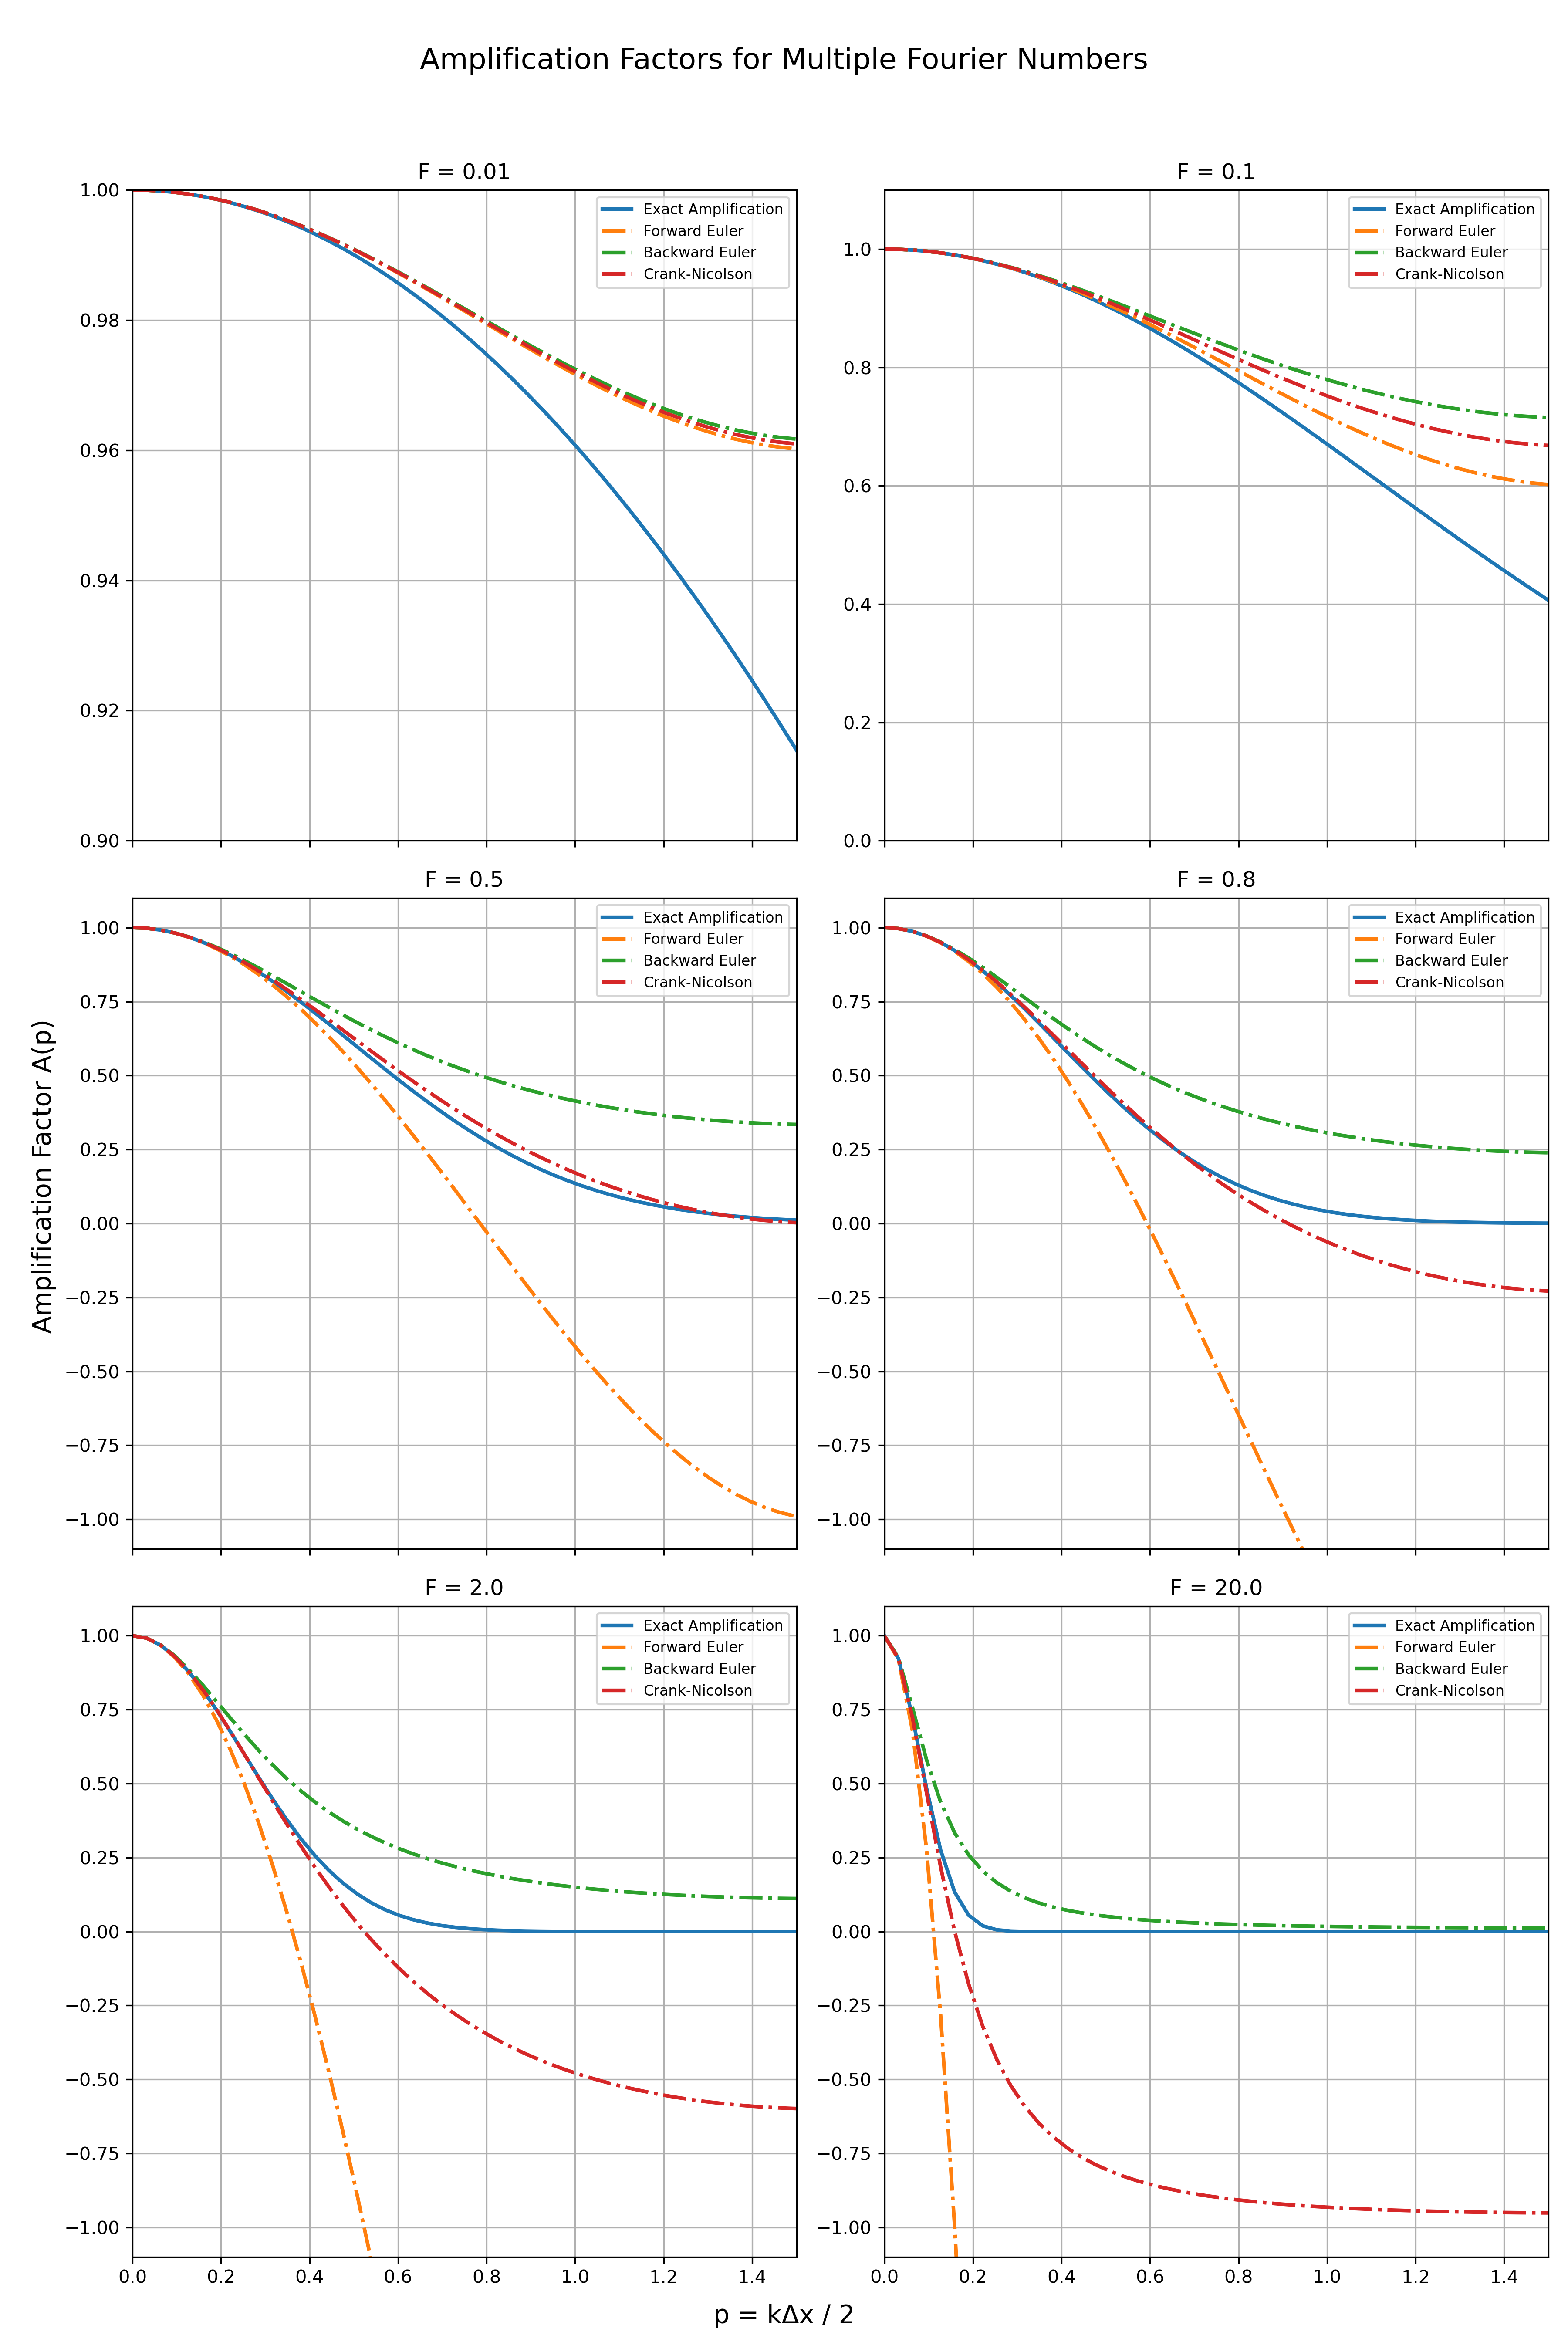
\includegraphics[width=\textwidth,height=\textheight,keepaspectratio=false]{amplification_factors_multiple_F_08}%amp_factors_multiple_F_and_schemes.png}
				}
				\caption{Amplification factors for different F and numerical schemes}
				\label{fig:amp_factors_multiple_F_and_schemes}
			\end{figure}
			
			\begin{comment}
			
			\begin{figure}[p] % 'p' ensures placement on a separate page
				\makebox[\textwidth]{ % Center horizontally
					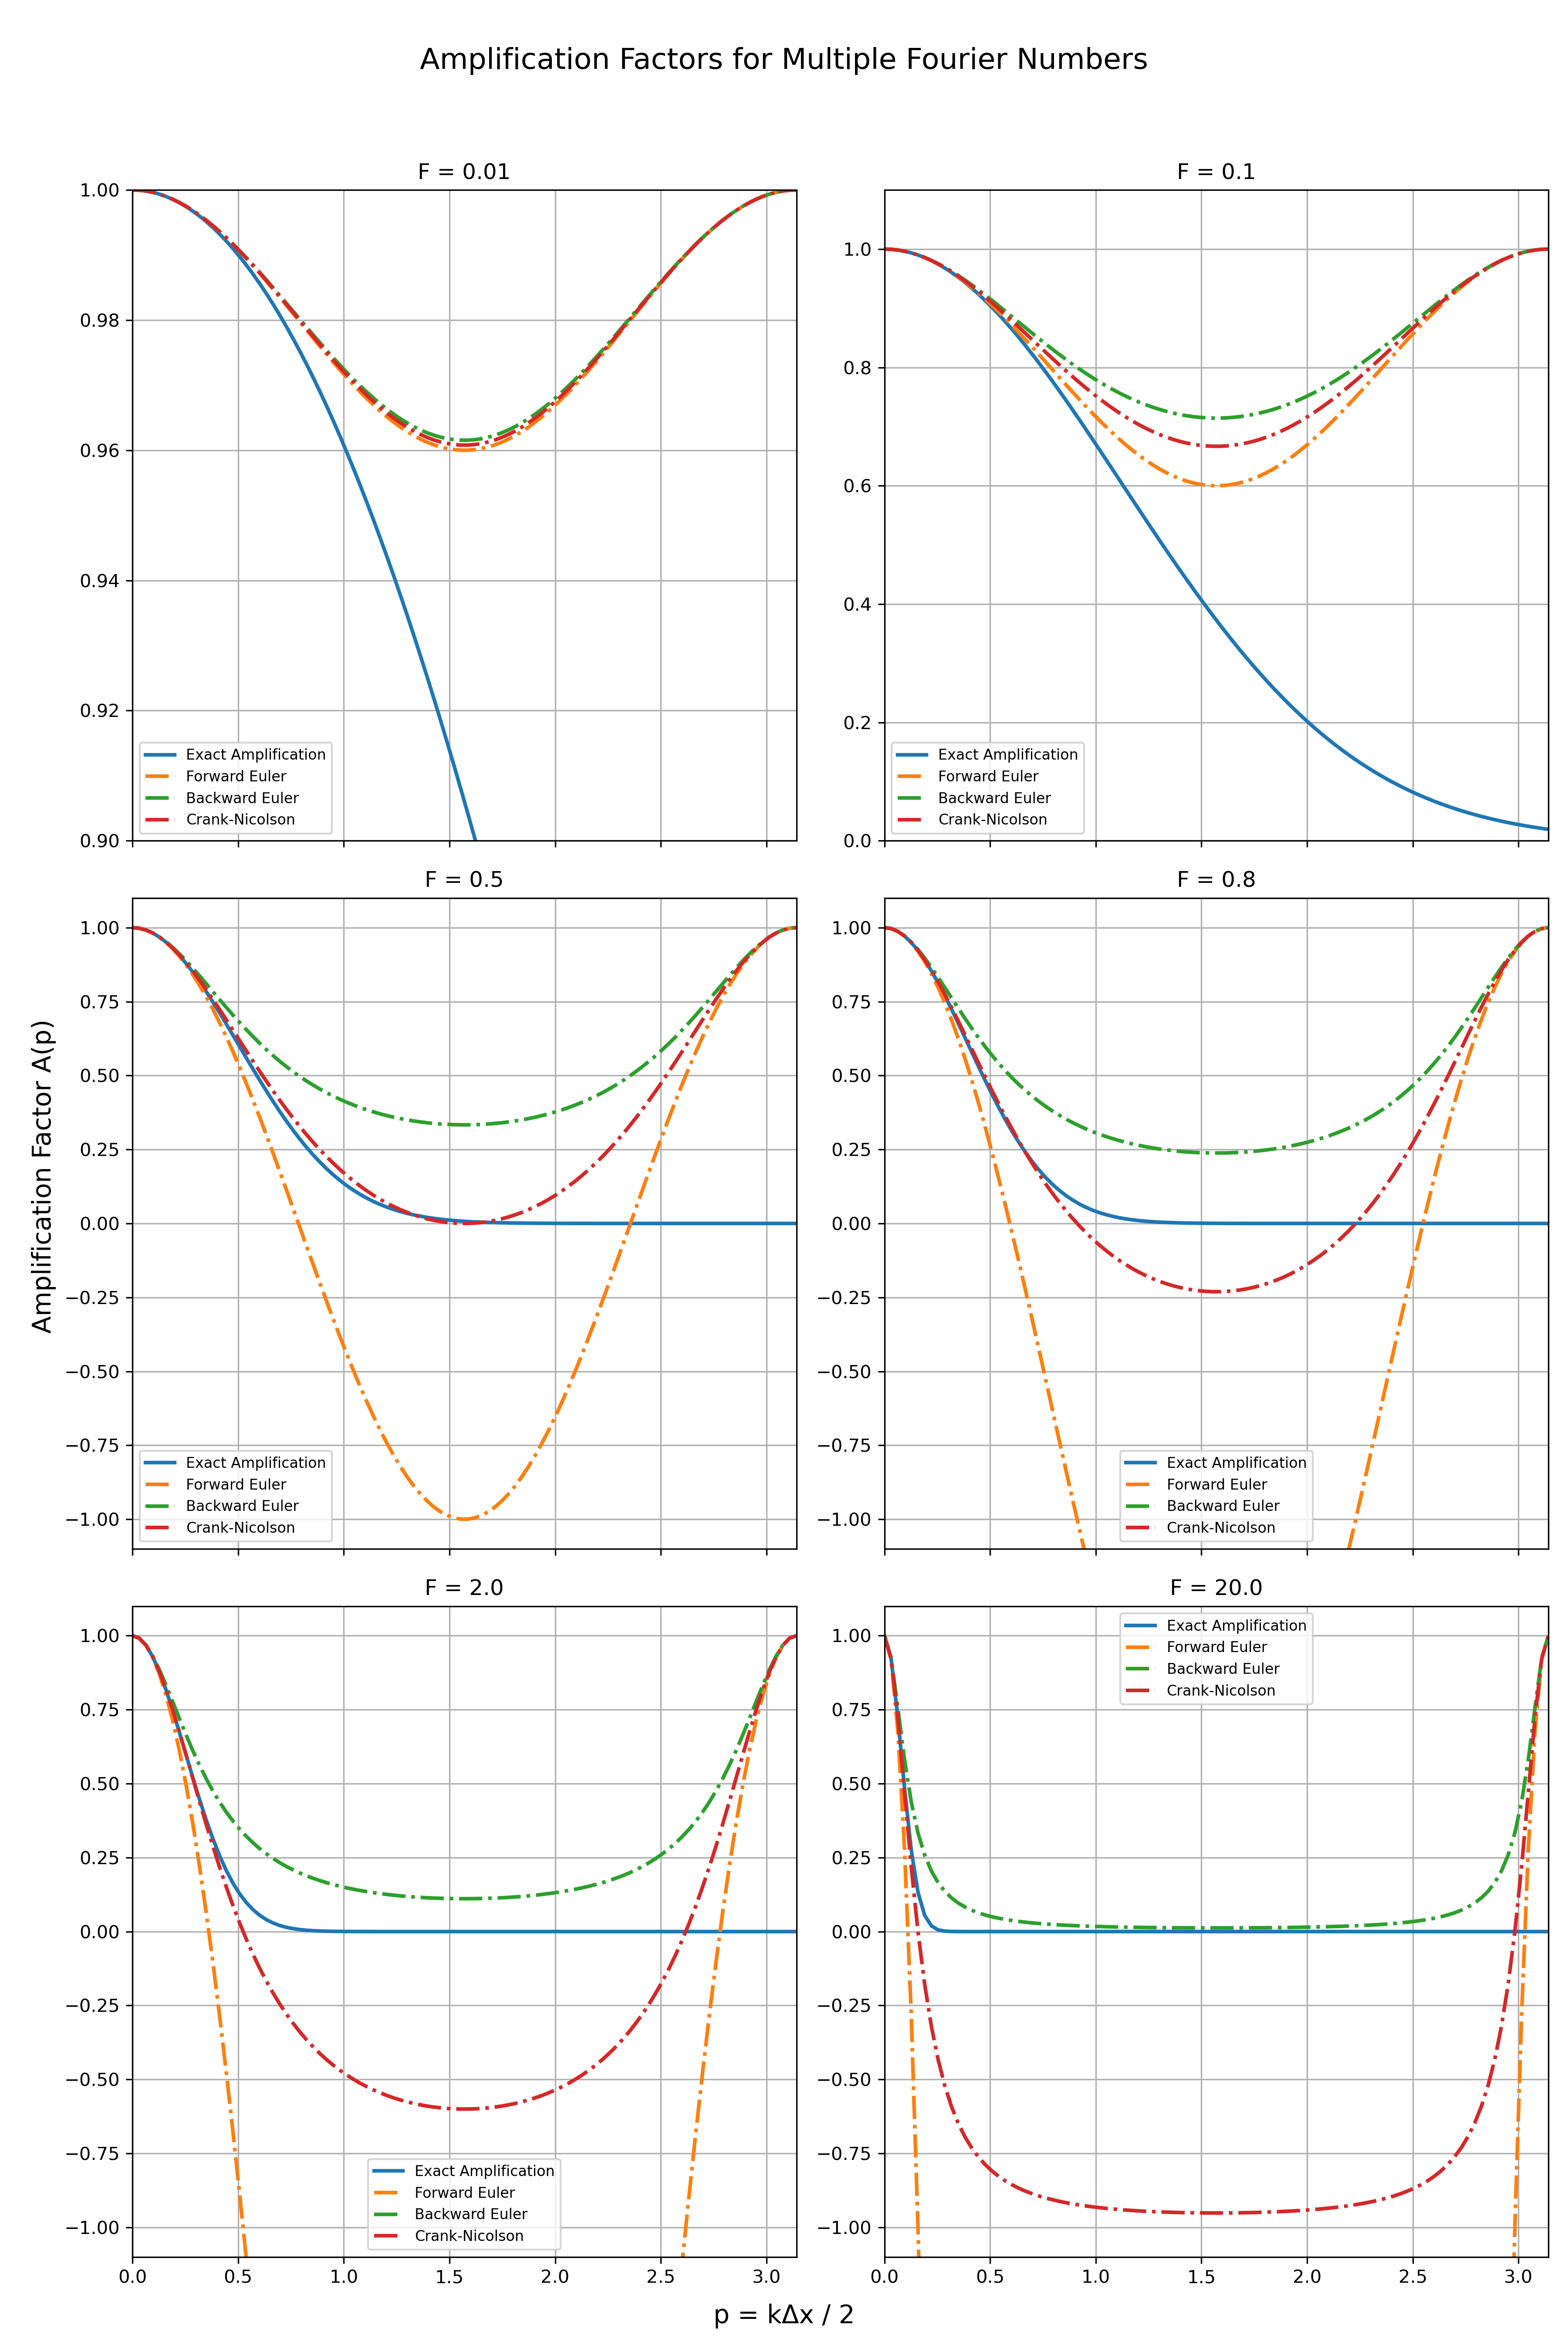
\includegraphics[width=\textwidth,height=\textheight,keepaspectratio=false]{amplification_factors_multiple_F}%amp_factors_multiple_F_and_schemes.png}
			}
			\caption{Amplification factors for different F and numerical schemes, max(p)}
			\label{fig:amp_factors_multiple_F_and_schemes}
			\end{figure}
				content...
			\end{comment}
	\newpage
	\section{2D Diffusion Solver Development}
		Mathematical formulation the diffusion equation in two spatial dimensions can be expressed as:
		\[
		\frac{\partial u}{\partial t} = \alpha \left( \frac{\partial^2 u}{\partial x^2} + \frac{\partial^2 u}{\partial y^2} \right) + f(x, y),
		\]
		in a rectangular domain \( (x, y) \in (0, L_x) \times (0, L_y), \; t \in (0, T] \).
		
		The boundary conditions are given as:
		\[
		u = 0 \quad \text{on the boundary},
		\]
		and the initial condition is specified as:
		\[
		u(x, y, 0) = I(x, y).
		\]
		
		\subsection{The Unified \(\theta\)-Rule Discretization}
		
			To solve the two-dimensional diffusion equation numerically, a general \(\theta\)-rule for time discretization is implemented. For the spatial derivatives, standard second-order accurate finite differences are used.
			
			\[
			\left[ D_t u \right]^{n+\frac{1}{2}} = \theta \left[ \alpha \left( D_x D_x u + D_y D_y u \right) + f \right]^{n+1}
			+ (1 - \theta) \left[ \alpha \left( D_x D_x u + D_y D_y u \right) + f \right]^n.
			\]
			
			Written explicitly, this becomes:
			\[
			\frac{u_{i,j}^{n+1} - u_{i,j}^n}{\Delta t} =
			\theta \alpha \left( \frac{u_{i-1,j}^{n+1} - 2u_{i,j}^{n+1} + u_{i+1,j}^{n+1}}{\Delta x^2} 
			+ \frac{u_{i,j-1}^{n+1} - 2u_{i,j}^{n+1} + u_{i,j+1}^{n+1}}{\Delta y^2} \right) 
			+ \theta f_{i,j}^{n+1}
			\]
			\[
			+ (1 - \theta) \alpha \left( \frac{u_{i-1,j}^n - 2u_{i,j}^n + u_{i+1,j}^n}{\Delta x^2}
			+ \frac{u_{i,j-1}^n - 2u_{i,j}^n + u_{i,j+1}^n}{\Delta y^2} \right)
			+ (1 - \theta) f_{i,j}^n.
			\]
			
			We rearrange to collect the unknowns on the left-hand side:
			\[
			u_{i,j}^{n+1} - \theta F_x \left( u_{i-1,j}^{n+1} - 2u_{i,j}^{n+1} + u_{i+1,j}^{n+1} \right)
			- \theta F_y \left( u_{i,j-1}^{n+1} - 2u_{i,j}^{n+1} + u_{i,j+1}^{n+1} \right)
			\]
			\[
			= (1 - \theta) F_x \left( u_{i-1,j}^n - 2u_{i,j}^n + u_{i+1,j}^n \right)
			+ (1 - \theta) F_y \left( u_{i,j-1}^n - 2u_{i,j}^n + u_{i,j+1}^n \right)
			+ \Delta t \theta f_{i,j}^{n+1} + \Delta t (1 - \theta) f_{i,j}^n + u_{i,j}^n,
			\]
			
			
			where:
			\[
			F_x = \frac{\alpha \Delta t}{\Delta x^2}, \quad F_y = \frac{\alpha \Delta t}{\Delta y^2},
			\]
			are the Fourier numbers in the \(x\)- and \(y\)-directions, respectively.
		
		\subsection{Construction of the System Matrix}
		
			The equations for the two-dimensional diffusion problem are coupled at the new time level \( n+1 \), requiring the solution of a system of linear equations \( A \mathbf{c} = \mathbf{b} \), where \( A \) is the coefficient matrix, \( \mathbf{c} \) is the vector of unknowns, and \( \mathbf{b} \) is the right-hand side.
			
			\paragraph{Boundary Conditions}
			For a mesh with \( N_x = 3 \) and \( N_y = 2 \), the boundary equations are:
			\[
			u_{i,j}^{n+1} = 0, \quad \text{for } i = 0, 1, 2, 3 \text{ and } j = 0, 2.
			\]
			This leaves two interior points: \( (i, j) = (1, 1) \) and \( (2, 1) \).
			
			\paragraph{Interior Equations}
			The equations at interior points are:
			\[
			u_{i,j}^{n+1} -  \theta F_x \left( u_{i-1,j}^{n+1} - 2u_{i,j}^{n+1} + u_{i+1,j}^{n+1} \right)
			-  \theta F_y \left( u_{i,j-1}^{n+1} - 2u_{i,j}^{n+1} + u_{i,j+1}^{n+1} \right)
			\]
			\[
			= (1-\theta) F_x \left( u_{i-1,j}^n - 2u_{i,j}^n + u_{i+1,j}^n \right)
			+ (1-\theta) F_y \left( u_{i,j-1}^n - 2u_{i,j}^n + u_{i,j+1}^n \right)
			+ \Delta t \theta f_{i,j}^{n+1} + \Delta t (1-\theta) f_{i,j}^n + u_{i,j}^n.
			\]
			
			\begin{comment}
			
			\paragraph{Single Index Numbering}
			To transform the mesh into a linear system, a mapping \( m(i, j) \) assigns a single index \( p \) to a mesh point \( (i, j) \):
			\[
			p = m(i, j) = j (N_x + 1) + i.
			\]
				content...
			\end{comment}
		
			
			\paragraph{Coefficient Matrix Structure}
			The entries of the coefficient matrix \( A \) for interior points are:
			\[
			A_{m(i,j), m(i,j)} = 1 + \theta (F_x + F_y), \quad
			A_{m(i,j), m(i-1,j)} = A_{m(i,j), m(i+1,j)} = -\theta F_x,
			\]
			\[
			A_{m(i,j), m(i,j-1)} = A_{m(i,j), m(i,j+1)} = -\theta F_y,
			\]
			with boundary entries:
			\[
			A_{m(i,j), m(i,j)} = 1, \quad \text{for boundary points.}
			\]
			
			The right-hand side vector \( \mathbf{b} \) includes contributions from the previous time step and the source term:
			\[
			b_{m(i,j)} = u_{i,j}^n + (1-\theta) \left[ F_x (u_{i-1,j}^n - 2u_{i,j}^n + u_{i+1,j}^n) + F_y (u_{i,j-1}^n - 2u_{i,j}^n + u_{i,j+1}^n) \right] + \Delta t \theta f_{i,j}^{n+1} + \Delta t (1-\theta) f_{i,j}^n.
			\]
			
			\paragraph{Sparsity of the Matrix}
			 The resulting matrix \( A \) is sparse, meaning that most of its elements are zero. The nonzero elements are arranged in a banded structure, confined to the main diagonal and a few adjacent diagonals. This banded sparsity significantly reduces the storage requirements and computational effort, as only the nonzero elements need to be considered during calculations.
			 For a mesh with \( N_x + 1 = N_y + 1 = N \), the fraction of nonzero elements is \( \frac{5}{N^2} \), demonstrating the efficiency of sparse matrix methods for solving such systems.
		
		\subsection{Algorithm for the Coefficient Matrix}
		
			
			
			\paragraph{General Approach}
			\begin{itemize}
				\item Initialize \( A \) as a zero matrix and \( b \) as a zero vector.
				\item Loop through all grid points \((i, j)\), where:
				\begin{itemize}
					\item \( i = 0, \ldots, N_x \): Points in the \( x \)-direction.
					\item \( j = 0, \ldots, N_y \): Points in the \( y \)-direction.
				\end{itemize}
				\item For each grid point \((i, j)\), compute the corresponding linear index \( p = j(N_x + 1) + i \).
				\item Determine whether \((i, j)\) is a boundary or interior point and update \( A \) and \( b \) accordingly.
			\end{itemize}
			To construct the coefficient matrix \( A \) and right-hand side vector \( b \), the following algorithm is applied:
			
			\begin{algorithm}
				\caption{Construction of Coefficient Matrix $A$ and Right-Hand Side $b$ for 2D Diffusion Equation}
				\begin{algorithmic}[1]
					\State Initialize matrix $A$ and vector $b$ with zeros.
					\For{$i = 0$ to $Nx$}
					\For{$j = 0$ to $Ny$}
					\State $p \gets j \cdot (Nx + 1) + i$ \Comment{Compute the linear index}
					\If{Point $(i, j)$ is on the boundary}
					\State $A_{p, p} \gets 1$
					\State $b_p \gets 0$
					\Else
					\State \Comment{Fill coefficients for interior points}
					\State $A_{p, m(i-1, j)} \gets F_x$
					\State $A_{p, m(i+1, j)} \gets F_x$
					\State $A_{p, m(i, j-1)} \gets F_y$
					\State $A_{p, m(i, j+1)} \gets F_y$
					\State $A_{p, p} \gets 1 + F_x + F_y$
					\State Compute $b_p$ based on the $\theta$-rule
					\EndIf
					\EndFor
					\EndFor
					
					\For{$j = 0$ to $Ny$}
					\Comment{Handle boundary lines and interior points separately}
					\State \Comment{Boundary: $j = 0$ (bottom boundary)}
					\For{$i = 0$ to $Nx$}
					\State $p \gets j \cdot (Nx + 1) + i$
					\State $A_{p, p} \gets 1$
					\EndFor
					\State \Comment{Interior lines: $1 \leq j < Ny$}
					\For{$i = 1$ to $Nx - 1$}
					\State $p \gets j \cdot (Nx + 1) + i$
					\State Fill $A_{p, m(i-1, j)}$, $A_{p, m(i+1, j)}$, $A_{p, m(i, j-1)}$, $A_{p, m(i, j+1)}$, $A_{p, p}$, and $b_p$
					\EndFor
					\State \Comment{Boundary: $j = Ny$ (top boundary)}
					\For{$i = 0$ to $Nx$}
					\State $p \gets j \cdot (Nx + 1) + i$
					\State $A_{p, p} \gets 1$
					\EndFor
					\EndFor
					
					\For{$i = 0$ to $Nx$}
					\Comment{Handle right-hand side vector $b$}
					\State \Comment{Boundary: $j = 0$ (bottom boundary)}
					\For{$j = 0$ to $Ny$}
					\State $p \gets j \cdot (Nx + 1) + i$
					\State $b_p \gets 0$
					\EndFor
					\State \Comment{Interior points: $1 \leq i < Nx$}
					\For{$j = 1$ to $Ny - 1$}
					\State $p \gets j \cdot (Nx + 1) + i$
					\State Compute $b_p$
					\EndFor
					\State \Comment{Boundary: $j = Ny$ (top boundary)}
					\For{$j = 0$ to $Ny$}
					\State $p \gets j \cdot (Nx + 1) + i$
					\State $b_p \gets 0$
					\EndFor
					\EndFor
					
				\end{algorithmic}
			\end{algorithm}
		\newpage
		
		\subsection{Implementation in Python}
		
		The function \texttt{theta\_diffusion\_2D} solves the 2D diffusion equation using the theta-rule method. The algorithm discretizes the spatial and temporal domains, assembles a coefficient matrix and right-hand side vector, and iteratively solves the system of equations at each time step. 
		
		\subsubsection{Function Signature and Parameters}
		\begin{lstlisting}
			def theta_diffusion_2D(
				I, f, alpha, Lx, Ly, Nx, Ny, dt, T, theta=0.5,
				U_0x=0, U_0y=0, U_Lx=0, U_Ly=0, user_action=None
				):
		\end{lstlisting}
		
		\noindent
		The solver takes the following arguments:
		\begin{itemize}
			\item $I$: Initial condition function $I(x, y)$.
			\item $f$: Source term function $f(x, y, t)$.
			\item $\alpha$: Diffusion coefficient.
			\item $L_x, L_y$: Dimensions of the spatial domain.
			\item $N_x, N_y$: Number of spatial grid points in the $x$ and $y$ directions.
			\item $dt$: Time step size.
			\item $T$: Total simulation time.
			\item $\theta$: Weighting parameter controlling the scheme:
			\begin{itemize}
				\item $\theta = 0$: Explicit (Forward Euler).
				\item $\theta = 0.5$: Semi-Implicit (Crank-Nicolson).
				\item $\theta = 1$: Fully implicit (Backward Euler).
			\end{itemize}
			\item $U_{0x}, U_{0y}, U_{Lx}, U_{Ly}$: Boundary conditions.
			\item \texttt{user\_action}: Optional function for visualization or output.
		\end{itemize}
		
		---
		
		\subsubsection{Setup and Initialization}
		\begin{lstlisting}
			import time
			t0 = time.time()  # Start measuring CPU time
			
			x = np.linspace(0, Lx, Nx + 1)  # Mesh points in x direction
			y = np.linspace(0, Ly, Ny + 1)  # Mesh points in y direction
			dx = x[1] - x[0]
			dy = y[1] - y[0]
			
			Nt = int(round(T / dt))  # Number of time steps
			t = np.linspace(0, Nt * dt, Nt + 1)  # Time array
		\end{lstlisting}
		
		\noindent
		%\textbf{Explanation:}
		\begin{itemize}
			\item Initializes the computational grid in space and time.
			\item $dx$ and $dy$ are the grid spacings in $x$ and $y$ directions:
			\[
			dx = \frac{L_x}{N_x}, \quad dy = \frac{L_y}{N_y}.
			\]
			\item $Nt$ is the total number of time steps:
			\[
			Nt = \frac{T}{dt}.
			\]
			\item $t$ is the time array containing all time steps.
		\end{itemize}
		
		---
		
		\subsubsection{Fourier Numbers and Source Term Handling}
		\begin{lstlisting}
			Fx = alpha * dt / dx**2
			Fy = alpha * dt / dy**2
			
			if f is None or f == 0:
				f = lambda x, y, t: 0
		\end{lstlisting}
		
		\noindent
		%\textbf{Explanation:}
		\begin{itemize}
			\item $F_x$ and $F_y$ are the Fourier numbers in $x$ and $y$ directions:
			\[
			F_x = \frac{\alpha \Delta t}{\Delta x^2}, \quad F_y = \frac{\alpha \Delta t}{\Delta y^2}.
			\]
			\item If no source term $f$ is provided, it defaults to zero everywhere.
		\end{itemize}
		
		---
		
		\subsubsection{Initializing Solution Arrays}
		\begin{lstlisting}
			u = np.zeros((Nx + 1, Ny + 1))  # Solution at the new time level
			u_n = np.zeros((Nx + 1, Ny + 1))  # Solution at the previous time level
			
			Ix = range(0, Nx + 1)
			Iy = range(0, Ny + 1)
			It = range(0, Nt + 1)
		\end{lstlisting}
		
		\noindent
		%\textbf{Explanation:}
		\begin{itemize}
			\item $u$ and $u_n$ store the solution at the current and previous time steps, respectively.
			\item $Ix$, $Iy$, and $It$ define the index ranges for grid points in $x$, $y$, and $t$.
		\end{itemize}
		
		---
		\begin{comment}
		
		\subsubsection{Handling Boundary Conditions}
		\begin{lstlisting}
			if not callable(U_0x):
				U_0x_val = float(U_0x)  # Convert scalar to float once
				U_0x = lambda t: U_0x_val
			if not callable(U_0y):
				U_0y_val = float(U_0y)  # Convert scalar to float once
				U_0y = lambda t: U_0y_val
			if not callable(U_Lx):
				U_Lx_val = float(U_Lx)  # Convert scalar to float once
				U_Lx = lambda t: U_Lx_val
			if not callable(U_Ly):
				U_Ly_val = float(U_Ly)  # Convert scalar to float once
				U_Ly = lambda t: U_Ly_val
		\end{lstlisting}
		
		\noindent
		%\textbf{Explanation:}
		\begin{itemize}
			\item Ensures all boundary conditions are treated as functions of time $t$, even if they are constants.
			\item For example, if $U_{0x} = c$ is a constant, it is converted to $U_{0x}(t) = c$.
		\end{itemize}
			content...
		\end{comment}
		---
		
		\subsubsection{Initial Condition Setup}
		\begin{lstlisting}
			# Load initial condition into u_n
			for i in Ix:
				for j in Iy:
					u_n[i, j] = I(x[i], y[j])
		\end{lstlisting}
		
		\noindent
		\begin{comment}
		
		%\textbf{Explanation:}
		\begin{itemize}
			\item Populates $u_n$ with the initial condition:
			\[
			u^n_{i,j} = I(x_i, y_j).
			\]
		\end{itemize}
			content...
		\end{comment}
		---
		
		\subsubsection{Matrix and RHS Vector Initialization}
		\begin{lstlisting}
			N = (Nx + 1) * (Ny + 1)  # Total number of unknowns
			A = np.zeros((N, N))  # Coefficient matrix
			b = np.zeros(N)  # Right-hand side vector
			
			m = lambda i, j: j * (Nx + 1) + i  # Linear index for (i, j)
		\end{lstlisting}
		
		\noindent
		\textbf{Explanation:}
		\begin{itemize}
			\item Initializes the coefficient matrix $A$ and RHS vector $\mathbf{b}$ for the linear system $A \mathbf{c} = \mathbf{b}$.
			\item The function $m(i, j)$ maps a 2D grid point $(i, j)$ to a 1D index $p$.
		\end{itemize}
		
		---
		
		\subsubsection{Matrix Assembly}
		\begin{lstlisting}
			# Boundary conditions and internal points
			for j in Iy:
				for i in Ix:
					p = m(i, j) # Linear index for the current point
					if j == 0 or j == Ny or i == 0 or i == Nx: # Boundary points
						A[p, p] = 1 
					else: # Internal points
						A[p, m(i, j - 1)] = -theta * Fy # y-direction lower
						A[p, m(i - 1, j)] = -theta * Fx # x-direction lower
						A[p, p] = 1 + 2 * theta * (Fx + Fy) # Center
						A[p, m(i + 1, j)] = -theta * Fx # x-direction upper
						A[p, m(i, j + 1)] = -theta * Fy # y-direction upper
		\end{lstlisting}
		
		\noindent
		\textbf{Explanation:}
		\begin{itemize}
			\item Boundary points enforce $A_{p,p} = 1$.
			\item Interior points use the finite difference stencil, as detailed earlier.
		\end{itemize}
		
		---
		
		\subsubsection{Time-Stepping Loop}
		
		\begin{lstlisting}
			# Time-stepping loop
			for n in It[:-1]:
				# Compute the right-hand side
				for j in Iy:
					for i in Ix:
						p = m(i, j)
						if j == 0:
							b[p] = U_0y(t[n + 1])  # Bottom boundary
						elif j == Ny:
							b[p] = U_Ly(t[n + 1])  # Top boundary
						elif i == 0:
							b[p] = U_0x(t[n + 1])  # Left boundary
						elif i == Nx:
							b[p] = U_Lx(t[n + 1])  # Right boundary
						else:
							b[p] = (
							u_n[i, j]
							+ (1 - theta)
							* (
							Fx * (u_n[i + 1, j] - 2 * u_n[i, j] + u_n[i - 1, j])
							+ Fy * (u_n[i, j + 1] - 2 * u_n[i, j] + u_n[i, j - 1])
							)
							+ theta * dt * f(i * dx, j * dy, (n + 1) * dt)
							+ (1 - theta) * dt * f(i * dx, j * dy, n * dt)
							)
							
						# Solve the linear system
						c = scipy.linalg.solve(A, b)
						
						# Fill u with the solution vector c
						for i in Ix:
							for j in Iy:
								u[i, j] = c[m(i, j)]
						
						if user_action is not None:
							user_action(u, x, xv, y, yv, t, n + 1)
						
						# Update u_n for the next time step
						u_n, u = u, u_n
		\end{lstlisting}
		
		\noindent
		\begin{comment}
		
		%\textbf{Explanation:}
		
		\paragraph{Time-Stepping Loop:}
		The main purpose of the loop is to iterate over time steps, updating the solution for the 2D diffusion equation. The iteration index $n$ corresponds to the current time step $t_n$, and the next time step is $t_{n+1}$.
		
		\paragraph{Right-Hand Side Computation:}
		The vector $\mathbf{b}$ is computed for all points $(i, j)$ on the spatial grid. Each point is mapped to its corresponding position in the 1D linear index $p$ using $p = j \cdot (Nx + 1) + i$, as explained in the coefficient matrix setup.
		
		\[
		b_p =
		\begin{cases}
			U_{0y}(t_{n+1}) & \text{if } j = 0 \text{ (bottom boundary)}, \\
			U_{Ly}(t_{n+1}) & \text{if } j = Ny \text{ (top boundary)}, \\
			U_{0x}(t_{n+1}) & \text{if } i = 0 \text{ (left boundary)}, \\
			U_{Lx}(t_{n+1}) & \text{if } i = Nx \text{ (right boundary)}, \\
			u_n[i, j] + (1-\theta) \cdot \text{spatial terms} + \text{source terms}, & \text{otherwise}.
		\end{cases}
		\]
		
		\noindent
		The detailed computation for interior points is as follows:
		
		\[
		\begin{aligned}
			b_p = & \; u_n[i, j] \\
			& + (1 - \theta) \cdot \bigg[
			F_x \cdot (u_n[i+1, j] - 2u_n[i, j] + u_n[i-1, j]) \\
			& \qquad + F_y \cdot (u_n[i, j+1] - 2u_n[i, j] + u_n[i, j-1])
			\bigg] \\
			& + \theta \cdot \Delta t \cdot f(x_i, y_j, t_{n+1}) \\
			& + (1 - \theta) \cdot \Delta t \cdot f(x_i, y_j, t_n).
		\end{aligned}
		\]
		
		Here:
		\begin{itemize}
			\item $F_x = \frac{\alpha \Delta t}{\Delta x^2}$ and $F_y = \frac{\alpha \Delta t}{\Delta y^2}$ are the Fourier numbers in the $x$ and $y$ directions.
			\item $u_n[i, j]$ is the value of $u$ at the current time step and grid point $(i, j)$.
			\item $\Delta t$ is the time step size.
			\item $f(x_i, y_j, t)$ is the source term evaluated at $(x_i, y_j)$ and time $t$.
		\end{itemize}
			content...
		\end{comment}
		
		\paragraph{Linear System Solution:}
		The linear system $A \mathbf{c} = \mathbf{b}$ is solved using \texttt{scipy.linalg.solve}, where:
		\begin{itemize}
			\item $A$ is the coefficient matrix representing the finite difference scheme.
			\item $\mathbf{b}$ is the right-hand side vector computed in the previous step.
			\item $\mathbf{c}$ is the solution vector, which is reshaped into the 2D solution array $u[i, j]$.
		\end{itemize}
		
		\paragraph{Solution Assignment:}
		The vector $\mathbf{c}$ is mapped back into the 2D array $u[i, j]$ using the inverse of the linear index $p = j \cdot (Nx + 1) + i$.
		
		\paragraph{User-Defined Actions:}
		If a \texttt{user\_action} function is provided, it is called with the updated solution $u$ and relevant parameters. This can be used for visualization, saving data, or other purposes.
		
		\paragraph{Updating for the Next Time Step:}
		The values of $u_n$ are updated to the current solution $u$, preparing for the next iteration. This corresponds to the time-stepping rule:
		\[
		u_n = u.
		\]
		
		This concludes one iteration of the time-stepping loop, and the process repeats until the final time step is reached.
			
		---
	
		\subsubsection{Finalize and Return}
		\begin{lstlisting}
			t1 = time.time()
			return t, t1 - t0
		\end{lstlisting}
		
		\noindent
		
		\begin{itemize}
			\item The simulation time is measured by calculating the difference between \texttt{t1} (end time) and \texttt{t0} (start time).
			\item Returns the time array \texttt{t} and the total CPU time.
		\end{itemize}
		
		---
		\begin{comment}
		
		\subsubsection{Summary of Key Steps}
		\begin{enumerate}
			\item Initialize the spatial and temporal grids, as well as the solution arrays.
			\item Handle boundary conditions and prepare the coefficient matrix $A$.
			\item Iterate over time steps, solving $A \mathbf{c} = \mathbf{b}$ at each step.
			\item Update the solution and invoke the \texttt{user\_action} function if provided.
		\end{enumerate}
		
		This solver efficiently handles the 2D diffusion equation using a dense matrix approach with the theta-rule. 
				content...
		\end{comment}
	
	\subsection{Verification Using the \texttt{quadratic\_solvers\_3} Function}
	
		This subsection demonstrates the usage of the function \texttt{quadratic\_solvers\_3}, which tests the solver for the 2D diffusion equation against an exact solution. The exact solution is quadratic in space and linear in time. The function verifies that the numerical solution matches the exact solution to within a specified tolerance.
		
		\begin{lstlisting}
			def quadratic_solvers_3(theta, Nx, Ny):
				"""Exact discrete solution of the scheme."""
				def u_exact(x, y, t):
					"""Exact solution."""
					return 5 * t * x * (Lx - x) * y * (Ly - y)
				
				def I(x, y):
					"""Initial condition."""
					return u_exact(x, y, 0)
					
				def f(x, y, t):
					"""Source term."""
					return 5 * x * (Lx - x) * y * (Ly - y) + 10 * a * t * (y * (Ly - y) + x * (Lx - x))
				
				# Domain parameters
				Lx = 0.75
				Ly = 1.5
				a = 3.5
				dt = 0.5
				T = 2  # Total simulation time
				
				def assert_no_error(u, x, xv, y, yv, t, n):
					"""Assert zero error at all mesh points."""
					xv, yv = np.meshgrid(x, y, indexing='ij')
					u_e = u_exact(xv, yv, t[n])
					diff = abs(u - u_e).max()
					tol = 1E-12
					msg = f"diff={diff:.6e}, step {n}, time={t[n]}"
					print(msg)
					assert diff < tol, msg
				
				# Test the solver with `theta_diffusion_2D`
				print(f"\nTesting theta={theta}, Nx={Nx}, Ny={Ny}")
					t, cpu = theta_diffusion_2D(
					I=I,
					f=f,
					alpha=a,
					Lx=Lx,
					Ly=Ly,
					Nx=Nx,
					Ny=Ny,
					T=T,
					dt=dt,
					theta=theta,
					U_0x=0,    # Explicit scalar boundary condition
					U_0y=0,    # Explicit scalar boundary condition
					U_Lx=0,    # Explicit scalar boundary condition
					U_Ly=0,    # Explicit scalar boundary condition
					user_action=assert_no_error,
					)
				
				print(f"Test completed for theta={theta}, Nx={Nx}, Ny={Ny}.")
				return t, cpu
		\end{lstlisting}
		
		\subsubsection{Mathematical Representation and Explanation}
		
		The \texttt{quadratic\_solvers\_3} function verifies the numerical solution by comparing it to the exact solution at every time step. Here are the key components of the function:
		
		\paragraph{Exact Solution.}
		The exact solution is given by:
		\[
		u(x, y, t) = 5t \cdot x(L_x - x) \cdot y(L_y - y),
		\]
		where \( L_x \) and \( L_y \) define the domain dimensions. This solution is linear in time and quadratic in space.
		
		\paragraph{Source Term.}
		The source term \( f(x, y, t) \) is derived by substituting the exact solution into the diffusion equation:
		\[
		f(x, y, t) = 5x(L_x - x)y(L_y - y) + 10\alpha t \cdot \left[ x(L_x - x) + y(L_y - y) \right].
		\]
		
		\paragraph{Initial Condition.}
		The initial condition corresponds to the exact solution evaluated at \( t = 0 \):
		\[
		I(x, y) = u(x, y, 0) = 0.
		\]
		
		\paragraph{Domain Parameters.}
		The simulation runs on a domain with:
		\begin{align*}
			L_x &= 0.75, & L_y &= 1.5, & \alpha &= 3.5.
		\end{align*}
		The total simulation time is \( T = 2 \), with a time step \( \Delta t = 0.5 \).
		
		\paragraph{Numerical Verification.}
		The function \texttt{assert\_no\_error} compares the numerical solution \( u \) with the exact solution \( u_e \) at every time step:
		\[
		\text{diff} = \max |u - u_e|, \quad \text{tol} = 10^{-12}.
		\]
		If the maximum error exceeds the tolerance, an exception is raised.
		
		\paragraph{Boundary Conditions.}
		Explicit scalar boundary conditions are applied:
		\[
		U_{0x} = U_{0y} = U_{Lx} = U_{Ly} = 0.
		\]
		
		\begin{comment}
		
		\paragraph{Execution.}
		The function calls the \texttt{theta\_diffusion\_2D} solver, passing the exact initial condition \( I(x, y) \), the derived source term \( f(x, y, t) \), and the domain parameters. It validates the numerical solution against the exact solution at every time step.
			content...
		\end{comment}
		
		\subsubsection{Testing the \texttt{quadratic\_solvers\_3} Function}
		
		To ensure the robustness of the solver, the \texttt{test\_quadratic\_solvers\_3} function runs multiple tests on the solver with varying grid sizes (\(N_x\) and \(N_y\)) and theta values.
		
		\begin{lstlisting}
			def test_quadratic_solvers_3():
				"""Test quadratic solution for various meshes and theta values."""
				for theta in [1, 0.5, 0]:  # Backward Euler, Crank-Nicolson, Forward Euler
					for Nx in range(2, 6, 2):
						for Ny in range(2, 6, 2):
						print(f"\n*** Testing for {Nx}x{Ny} mesh with theta={theta}")
						quadratic_solvers_3(theta, Nx, Ny)
		\end{lstlisting}
		
		\paragraph{Description of the Test Function.}
		The \texttt{test\_quadratic\_solvers\_3} function iterates through combinations of:
		\begin{itemize}
			\item \textbf{Theta values:} \( \theta = 1 \) (Backward Euler), \( \theta = 0.5 \) (Crank-Nicolson), and \( \theta = 0 \) (Forward Euler).
			\item \textbf{Grid sizes:} Mesh resolutions are varied with \( N_x \) and \( N_y \) taking values in the range \( [2, 6] \) with a step of 2.
		\end{itemize}
		
		\begin{comment}
		
		\paragraph{Execution Steps.}
		For each combination of \(\theta\), \(N_x\), and \(N_y\):
		\begin{enumerate}
			\item The \texttt{quadratic\_solvers\_3} function is called to run the solver with the specified parameters.
			\item The solver compares the numerical solution to the exact solution for every time step, ensuring the error remains below a tolerance level (\(10^{-12}\)).
			\item Results, including any discrepancies and CPU time, are printed for each test.
		\end{enumerate}
		
		\paragraph{Output.}
		For each test case, the function outputs:
		\begin{itemize}
			\item The mesh size and \(\theta\) value being tested.
			\item The maximum error and corresponding time step if discrepancies are found.
			\item A summary indicating the completion of each test case.
		\end{itemize}
			content...
		\end{comment}
				
		The \texttt{test\_quadratic\_solvers\_3} function produces the following output when executed. Each block corresponds to a specific combination of mesh size (\(N_x, N_y\)) and the \(\theta\)-value (1, 0.5, or 0). The outputs display the difference (\texttt{diff}) between the numerical solution and the exact solution at every time step.
		
		\begin{lstlisting}
			*** Testing for 2x2 mesh with theta=1
			
			Testing theta=1, Nx=2, Ny=2
			diff=0.000000e+00, step 0, time=0.0
			diff=1.297325e-16, step 1, time=0.5
			diff=2.594651e-16, step 2, time=1.0
			diff=4.989808e-16, step 3, time=1.5
			diff=5.189301e-16, step 4, time=2.0
			Test completed for theta=1, Nx=2, Ny=2.
			
			*** Testing for 2x4 mesh with theta=1
			
			Testing theta=1, Nx=2, Ny=4
			diff=0.000000e+00, step 0, time=0.0
			diff=2.359146e-16, step 1, time=0.5
			diff=4.718293e-16, step 2, time=1.0
			diff=1.104299e-15, step 3, time=1.5
			diff=9.436586e-16, step 4, time=2.0
			Test completed for theta=1, Nx=2, Ny=4.
			
			...
			
			*** Testing for 4x4 mesh with theta=0
			
			Testing theta=0, Nx=4, Ny=4
			diff=0.000000e+00, step 0, time=0.0
			diff=0.000000e+00, step 1, time=0.5
			diff=0.000000e+00, step 2, time=1.0
			diff=0.000000e+00, step 3, time=1.5
			diff=0.000000e+00, step 4, time=2.0
			Test completed for theta=0, Nx=4, Ny=4.
			PASSED
		\end{lstlisting}
		
		
		
	\newpage
	\section*{Acknowledgments}
	
	I acknowledge the use of ChatGPT for writing assistance and code debugging in the preparation of this document.
	
			
		
	
		
			
		
		
\end{document}
